\documentclass[./main.tex]{subfiles} 
\begin{document}

\section{Adaptive Signal Processing}

\subsection{The Least Mean Squares (LMS) Algorithm}

\subsubsection{Correlation Matrix}
The autocorrelation matrix is been defined as $ R \equiv E \begin{bmatrix} \mathbf{x}[n] \mathbf{x}^T[n] \end{bmatrix} $, where $ \mathbf{x}(n) = [x(n-1), x(n-2)]^T $

\begin{equation} \label{eq:3_1_a_R}
R = 
\begin{bmatrix}
R_{xx}(0) & R_{xx}(1) \\
R_{xx}(1) & R_{xx}(0)
\end{bmatrix}
= E \left\{ \begin{bmatrix}
x^2[n-1] & x[n-1] x[n-2] \\
x[n-1] x[n-2] & x^2[n-2]
\end{bmatrix} \right\}
= \begin{bmatrix}
E \{ x^2[n-1] \} & E \{ x[n-1] x[n-2] \} \\
E \{ x[n-1] x[n-2] \} & E \{ x^2[n-2] \}
\end{bmatrix}
\end{equation}

We note that $x^2[n-1] = x^2[n-2] $ since this simply represents a shift in the time domain but will not change the expected value. 

We can square $x[n-1]$ to give us the expected value of the diagonals:
\begin{subequations}
\begin{align}
E[x^2[n-1]] &= E[ a_{1}^2 x^2[n-2] + a_{2}^2 x^2[n-3] + 2 a_{1} a_{2} x[n-1] x[n-2] + \eta[n-1](a_{1} x[n-2] + a_{2}x[n-3]) \\ \nonumber &\qquad + \eta^2[n-1] ] \\	
E[x^2[n-1]] &= E[ a_{1}^2 x^2[n - 2]] + E[ a_{2}^2 x^2[n-3]] + E[ 2 a_{1} a_{2} x[n-1] x[n-2]] + 
\sigma^2 \\
R_{xx}(0) = E[x^2[n-1]] &= a_1^2 R_{xx}(0) + a_2^2 R_{xx}(0) + 2 a_{1} a_{2} R_{xx}(1) + \sigma^2
\end{align}
\end{subequations}

We get to the last line using the equality mentioned above, and we can see the make up of $R_{xx}(1)$ in equation \ref{eq:3_1_a_R}. We can conduct a similar process for $R_{xx}(1)$:

\begin{subequations}
\begin{align}
E[x[n-1]x[n-2]] &= E[ a_1 x^2[n - 2] + a_2 x[n-3]x[n-2] + \eta[n-1]x[n-2] ] \\
R_{xx}(1) = E[x[n-1]x[n-2]] &= a_1 R_{xx}(0) + a_2 R_{xx}(1) + 0
\end{align}
\end{subequations}

We then solve these two equations for $ R_{xx}(0) $ and $ R_{xx}(1) $, to determine that the autocorrelation matrix is 
$$ R = \begin{bmatrix}
\frac{25}{27} & \frac{25}{54} \\[0.3em]
 \frac{25}{54} & \frac{25}{27}
\end{bmatrix}
$$

In order for the filter to converge to the correct parameters, we must satisfy the bounds $ 0 < \mu < \frac{2}{\lambda_{max}} $. In this case, our eigenvalues are $\frac{25}{18}$ and $\frac{25}{54}$. Thus we know that $ 0 < \mu < \frac{108}{25} $ for the LMS to converge in the mean.

\subsubsection{Implemented LMS Filter} \label{sec:3_1_b}
100 iterations of the AR Process $ x[n] = 0.1 x[n-1] + 0.8 x[n-2] + \eta[n] $ have been generated, with 1000 samples per iteration. Figure \ref{fig:q3_1_b_indiv} shows one trial of this filter, whist figure \ref{fig:q3_1_b} shows the mean error taken across 100 iterations. We can see that 100 iterations shows a much clearer trend in the error decreasing and becoming steady at around 300 iterations in.

\begin{figure}[h]
	\centering 
 	\resizebox{\textwidth}{!}{% This file was created by matlab2tikz v0.4.7 (commit e8e34ce6bed2236de660d19205fcab087937605e) running on MATLAB 8.3.
% Copyright (c) 2008--2014, Nico Schlömer <nico.schloemer@gmail.com>
% All rights reserved.
% Minimal pgfplots version: 1.3
% 
% The latest updates can be retrieved from
%   http://www.mathworks.com/matlabcentral/fileexchange/22022-matlab2tikz
% where you can also make suggestions and rate matlab2tikz.
% 
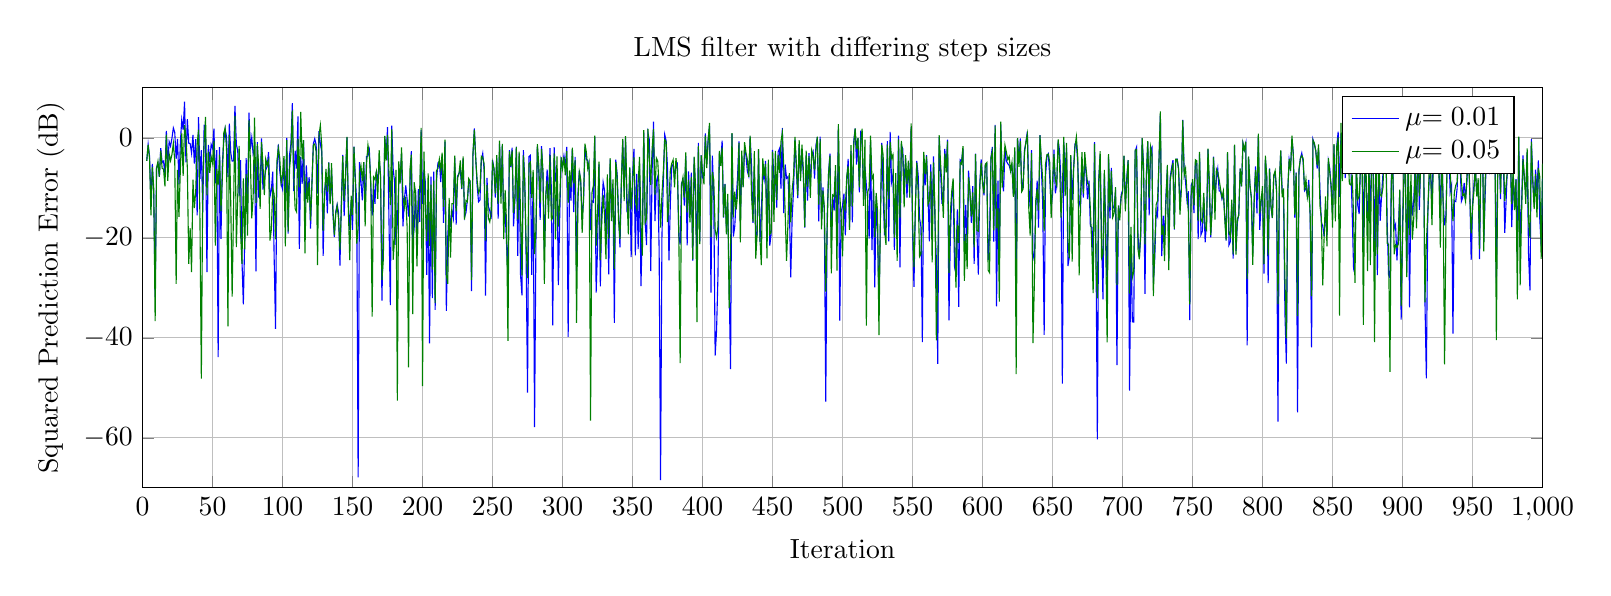
\begin{tikzpicture}

\begin{axis}[%
width=7in,
height=2in,
unbounded coords=jump,
scale only axis,
xmin=0,
xmax=1000,
xlabel={Iteration},
xmajorgrids,
ymin=-70,
ymax=10,
ylabel={Squared Prediction Error (dB)},
ymajorgrids,
title={LMS filter with differing step sizes},
legend style={draw=black,fill=white,legend cell align=left}
]
\addplot [color=blue,solid]
  table[row sep=crcr]{1	-inf\\
2	-inf\\
3	-4.59507082620591\\
4	-1.29996298596598\\
5	-3.70388331513567\\
6	-12.886796582078\\
7	-5.21161423976009\\
8	-11.4515929637692\\
9	-31.8370688452581\\
10	-5.99162122660154\\
11	-5.08424174660262\\
12	-7.79254593632003\\
13	-2.06806015100985\\
14	-4.92051303110294\\
15	-4.64612437362596\\
16	-7.36334277057199\\
17	1.40876675529917\\
18	-5.0262432391268\\
19	-0.758097027471307\\
20	-1.6496687842333\\
21	-0.077601116516787\\
22	1.97568414911764\\
23	1.10298527821058\\
24	-4.19253733201039\\
25	-0.198870346518106\\
26	-9.3095623607669\\
27	-1.01821155998611\\
28	3.6024438963203\\
29	1.6173802853813\\
30	7.22941099683327\\
31	-4.90031115684373\\
32	3.7503490465052\\
33	-1.0576737892293\\
34	-1.13233545410099\\
35	-3.03883378331891\\
36	0.573129369513038\\
37	-5.13192022683942\\
38	-0.276296218095252\\
39	-15.5128888879724\\
40	4.1398369269964\\
41	-8.17794661983596\\
42	-2.44369493494699\\
43	-14.8946763118055\\
44	2.65976655029787\\
45	-0.0394474379340101\\
46	-26.8684613523647\\
47	-1.42133766862283\\
48	-4.82857983328491\\
49	-1.30330785168854\\
50	-2.10558373460676\\
51	1.83122424331736\\
52	-9.07613523964419\\
53	-2.43586414265314\\
54	-43.8608087336864\\
55	-1.8442658460936\\
56	-20.2101840746231\\
57	-5.11221560134833\\
58	-0.739777467831388\\
59	1.75173115316697\\
60	0.231989354962519\\
61	-7.85790934623202\\
62	2.83678802826973\\
63	-2.98120455648551\\
64	-4.63760333820862\\
65	-4.60747291274579\\
66	6.38720782860191\\
67	-1.30263365227467\\
68	-2.59934307167544\\
69	-11.651066347851\\
70	-4.44070447113303\\
71	-24.3951070902113\\
72	-33.2958131455893\\
73	-20.1564571010961\\
74	-4.06092041390022\\
75	-15.2571950153253\\
76	5.03557130376121\\
77	-2.20505859308837\\
78	0.0543752516346717\\
79	-3.26661775112839\\
80	-2.30448933256956\\
81	-26.7185809941387\\
82	-0.834947144094049\\
83	-11.9348680897793\\
84	-10.1041576485053\\
85	-0.0983277583617844\\
86	-10.3460119082907\\
87	-8.24348146730097\\
88	-6.42732422694919\\
89	-5.74574071803219\\
90	-2.83501623014551\\
91	-11.7501929701949\\
92	-10.4795077260658\\
93	-6.73708069559175\\
94	-23.864291145364\\
95	-38.1993688773272\\
96	-6.09531401969005\\
97	-1.31943322728795\\
98	-6.54184797217457\\
99	-9.24243669632859\\
100	-10.2514267660012\\
101	-4.35629192220219\\
102	-13.3807838448117\\
103	0.0183787725011844\\
104	-19.152998673932\\
105	-3.43071743111616\\
106	-1.11428963801003\\
107	6.92598566526701\\
108	-10.671238192262\\
109	-2.5763252146889\\
110	-6.14809048565763\\
111	4.28900252463904\\
112	-22.1820323251344\\
113	-3.87733164372634\\
114	-9.19193006295974\\
115	-0.50820181437446\\
116	-13.6797773066692\\
117	-5.50277846404101\\
118	-11.104973275357\\
119	-7.8581784814733\\
120	-18.167470554977\\
121	-8.86388988270849\\
122	-1.17932001354982\\
123	-0.173843892636093\\
124	-1.41001109031989\\
125	-11.1351654408496\\
126	1.32609109963583\\
127	-1.16111425898\\
128	-2.76552856078371\\
129	-23.5981420714182\\
130	-10.6510614426644\\
131	-8.17233603411163\\
132	-15.07750206477\\
133	-4.91182925626672\\
134	-13.1109926636608\\
135	-6.3650256200269\\
136	-15.2076948811646\\
137	-19.8704542331295\\
138	-14.7754553992367\\
139	-13.3283581467692\\
140	-14.9293129240127\\
141	-25.5340869613823\\
142	-13.0121406171393\\
143	-3.40170879957216\\
144	-15.6306722974278\\
145	-8.3444023512049\\
146	0.0993009897631158\\
147	-13.297418621087\\
148	-18.3912674721723\\
149	-12.8095607365625\\
150	-18.4180152488787\\
151	-1.77314047203756\\
152	-8.00979329271622\\
153	-13.0798758610286\\
154	-67.8798107293025\\
155	-4.8713240947399\\
156	-8.62353014193708\\
157	-12.4956045813881\\
158	-4.8789965668519\\
159	-13.6827434845321\\
160	-3.69847656875362\\
161	-3.65416040114594\\
162	-2.47866388854382\\
163	-9.27219663908088\\
164	-15.5569454846821\\
165	-9.18269700077577\\
166	-13.2004768376506\\
167	-6.59536159387419\\
168	-9.32623776602284\\
169	-4.35391172388237\\
170	-7.45588773925131\\
171	-32.5646848152241\\
172	-15.7648371832139\\
173	0.290314107379467\\
174	-3.80533935492875\\
175	2.16206068938495\\
176	-16.2097483783635\\
177	-33.4381878005289\\
178	2.42970182112264\\
179	-6.13827213232283\\
180	-8.78183551030334\\
181	-21.4209022307097\\
182	-17.0412750064657\\
183	-8.97365984758658\\
184	-7.91276035077917\\
185	-3.21215558211807\\
186	-17.6906391102931\\
187	-12.4179301429368\\
188	-9.53250601887263\\
189	-12.2898472545387\\
190	-15.7302754663766\\
191	-9.49431646292227\\
192	-2.67296133362224\\
193	-20.7538936228713\\
194	-18.1525034084186\\
195	-10.4251631852447\\
196	-21.0081519792554\\
197	-10.254204952508\\
198	-16.7954087768511\\
199	1.57208708557949\\
200	-13.1841153849734\\
201	-6.34799004651346\\
202	-8.89470144548437\\
203	-27.4103919291639\\
204	-10.3470266018799\\
205	-41.0806085382544\\
206	-7.76301208371989\\
207	-32.0349062880966\\
208	-6.7327939113944\\
209	-34.3969084998931\\
210	-8.28871591620671\\
211	-5.01886041498538\\
212	-4.71853660706931\\
213	-8.82505129259185\\
214	-3.51010923435167\\
215	-16.9963362896896\\
216	-0.730528882716501\\
217	-34.6196189079352\\
218	-19.7688721520734\\
219	-13.8765771507028\\
220	-17.8131518378593\\
221	-14.6634275490892\\
222	-16.0848299004548\\
223	-4.02587569361607\\
224	-17.3354494602711\\
225	-7.69915922620534\\
226	-7.07420493402448\\
227	-6.43256957204218\\
228	-10.2499480993552\\
229	-4.09385110283117\\
230	-15.8624865883882\\
231	-14.954989250737\\
232	-12.5134906300228\\
233	-8.99234868899662\\
234	-8.74926368569967\\
235	-30.6635886562186\\
236	-3.49476079151981\\
237	1.87692346468992\\
238	-4.18683889744427\\
239	-9.5559126140898\\
240	-12.7853084356965\\
241	-12.4270117494065\\
242	-4.56164412282348\\
243	-3.11649965297617\\
244	-6.4640977568059\\
245	-31.5667969584002\\
246	-7.9842704350142\\
247	-13.7292998292345\\
248	-14.5424244544422\\
249	-16.2279056472344\\
250	-4.41152282722257\\
251	-6.18537695238337\\
252	-11.9244805502852\\
253	-4.10245450391466\\
254	-16.1558960757809\\
255	-1.21847923362777\\
256	-11.6163037287194\\
257	-1.40743926494729\\
258	-17.3185386950072\\
259	-14.7877704292476\\
260	-21.234889571928\\
261	-27.7414751415603\\
262	-2.44167960718865\\
263	-5.83147354970486\\
264	-1.94338610639582\\
265	-17.7195805791287\\
266	-12.1778983044332\\
267	-1.74624119572146\\
268	-23.5950554512173\\
269	-3.09265685071966\\
270	-27.4090947400917\\
271	-31.4848663903897\\
272	-2.469115747857\\
273	-8.21086296044095\\
274	-24.3761309060737\\
275	-50.9309983521741\\
276	-3.73342903937243\\
277	-3.48599763691293\\
278	-27.3803033529927\\
279	-7.9197297715811\\
280	-57.8336011979566\\
281	-20.1044662510308\\
282	-1.62924795565196\\
283	-6.52224671548055\\
284	-16.4178408997187\\
285	-1.63531266213463\\
286	-7.049154576417\\
287	-22.6913949630415\\
288	-11.7995710988729\\
289	-6.33149462795096\\
290	-13.8445162269544\\
291	-2.033115959314\\
292	-10.214550246611\\
293	-37.4794256414866\\
294	-1.85329762372136\\
295	-8.75732207127788\\
296	-6.62990334596757\\
297	-29.4376381613258\\
298	-15.4224345685412\\
299	-4.38626569475822\\
300	-5.57282360658109\\
301	-3.54999256460616\\
302	-5.60055661953875\\
303	-1.79193704050829\\
304	-39.7806079213807\\
305	-7.64824348894368\\
306	-12.5426513281241\\
307	-2.17789945825479\\
308	-14.8405457588761\\
309	-3.81946842826283\\
310	-26.663552504303\\
311	-11.1256911677689\\
312	-6.49047959791645\\
313	-9.11794370343059\\
314	-15.6892526371147\\
315	-12.7992989995148\\
316	-1.77578442645775\\
317	-4.34970961006816\\
318	-4.48446596321813\\
319	-6.12356035243434\\
320	-18.4663190660257\\
321	-12.5937084556932\\
322	-12.8499281501326\\
323	0.134504841403184\\
324	-30.9515249949078\\
325	-22.0388073875331\\
326	-5.28875253141051\\
327	-29.723246827461\\
328	-13.9147915126818\\
329	-8.88979378957893\\
330	-10.5320046110287\\
331	-18.5165653404073\\
332	-11.0609292076673\\
333	-27.3054484804337\\
334	-4.28227567648723\\
335	-14.9241250826485\\
336	-10.0043263230464\\
337	-37.0130881420234\\
338	-4.37246630658153\\
339	-7.26399436249821\\
340	-14.8434148010706\\
341	-21.8793792859966\\
342	-9.45580093095956\\
343	-0.559489052786781\\
344	-10.626668027507\\
345	0.0129315707530535\\
346	-14.6851468194501\\
347	-15.3193374109357\\
348	-6.12558360255809\\
349	-23.8503853354557\\
350	-7.6322770221229\\
351	-2.21046023269715\\
352	-23.5146177835239\\
353	-7.22302901743624\\
354	-22.2691387721479\\
355	-6.26649583247766\\
356	-29.6443851567446\\
357	-18.2473211824487\\
358	1.04982984971172\\
359	-16.6178353037298\\
360	-21.4331081748009\\
361	0.971111150022873\\
362	-0.386985153461473\\
363	-26.6260658910693\\
364	-6.21568263451509\\
365	3.24528470398526\\
366	-16.654678204431\\
367	-8.74410983119098\\
368	-7.73779060519475\\
369	-22.5970694892614\\
370	-68.4469019816751\\
371	-19.5353467588415\\
372	-8.59866069349975\\
373	0.658040388164451\\
374	-0.609359314445117\\
375	-6.34160738146867\\
376	-24.524191047539\\
377	-13.0186888297633\\
378	-5.29764461668775\\
379	-5.61178920306852\\
380	-8.02663249324909\\
381	-4.80507716175149\\
382	-5.0367922652333\\
383	-19.600287390056\\
384	-21.3555994885052\\
385	-9.11700423261428\\
386	-8.38759234391449\\
387	-13.5354160994604\\
388	-3.63369643485395\\
389	-21.5215489864056\\
390	-6.69524651519009\\
391	-14.0352044412132\\
392	-6.97299698142079\\
393	-24.5437723342562\\
394	-3.89794360118936\\
395	-11.4007279363398\\
396	-24.8635622808819\\
397	-0.989728166179697\\
398	-20.7151684821471\\
399	-3.44957700946648\\
400	-7.89217444923396\\
401	-7.4512907946588\\
402	0.897049616552637\\
403	-5.21647046361236\\
404	-0.260277362193214\\
405	2.35688640880273\\
406	-30.9401730031022\\
407	-3.55742416368125\\
408	-11.296960226021\\
409	-43.5575009659946\\
410	-38.5716970565132\\
411	-27.6790599041766\\
412	-3.65044722916638\\
413	-4.74205554608764\\
414	-0.546083345850634\\
415	-15.9279673627633\\
416	-9.215540787427\\
417	-17.9939008396808\\
418	-12.9298854771972\\
419	-29.4591632173433\\
420	-46.2324028684693\\
421	0.872144235007382\\
422	-19.7383201399374\\
423	-17.7338618408133\\
424	-12.3400541916129\\
425	-7.91933368859598\\
426	-0.724951334866135\\
427	-16.9438322294593\\
428	-3.87322146809172\\
429	-9.77766156164657\\
430	-2.2799497575516\\
431	-3.46232804437846\\
432	-6.66975950021396\\
433	-7.64343244956849\\
434	0.265543639754774\\
435	-5.61272342064353\\
436	-17.0005461011555\\
437	-6.43514883117215\\
438	-19.3293337078133\\
439	-19.4102556923633\\
440	-2.51619356556718\\
441	-20.8157786757831\\
442	-15.059990349752\\
443	-6.50971397149091\\
444	-8.36142565433981\\
445	-4.60492032628457\\
446	-16.8329011943879\\
447	-7.31184564338407\\
448	-21.5554017203759\\
449	-19.2287822796231\\
450	-2.41758081503257\\
451	-8.68711230220087\\
452	-7.40243215603317\\
453	-13.9690477824568\\
454	-2.81684443908056\\
455	-2.12802720993685\\
456	-10.1360977786818\\
457	1.95712346627217\\
458	-15.0495361171828\\
459	-5.33223691626302\\
460	-8.0822792755122\\
461	-7.75011648932619\\
462	-13.5099209237612\\
463	-27.9051087369194\\
464	-15.9524237906848\\
465	-10.4588298894738\\
466	-0.374689457951622\\
467	-6.34337401071064\\
468	-12.0623033859673\\
469	-1.28982523731276\\
470	-7.15720053986975\\
471	-3.20341640882774\\
472	-7.33437632689617\\
473	-17.9611041005778\\
474	-3.46930370543498\\
475	-12.5538046795972\\
476	-3.04101371975908\\
477	-9.20069732172808\\
478	-3.42541422572739\\
479	-2.72345271534146\\
480	-8.1282286315345\\
481	-1.47244212886749\\
482	0.165360741722727\\
483	-16.6788900603673\\
484	0.231182230266583\\
485	-16.3361804489302\\
486	-9.91726254832736\\
487	-15.0525583598902\\
488	-52.736230493891\\
489	-15.9025058786515\\
490	-7.09745032673951\\
491	-3.15318036805746\\
492	-20.4031897042768\\
493	-12.1211281856933\\
494	-14.5585372286106\\
495	-6.56361969993684\\
496	-21.6914194284372\\
497	2.30577660084875\\
498	-36.5417851588361\\
499	-14.8862425900649\\
500	-13.553063569923\\
501	-11.1677813226703\\
502	-19.4993084004511\\
503	-8.82882928953749\\
504	-4.19438031309641\\
505	-17.8844070629149\\
506	-2.59151300868696\\
507	-16.9236679856363\\
508	-0.675193300907349\\
509	1.88587207518606\\
510	-5.36833986435831\\
511	-0.0793074678597081\\
512	-10.9236823934515\\
513	1.45550837958505\\
514	-0.534628893516546\\
515	-12.3578339926104\\
516	-5.76091845114609\\
517	-9.52070462835327\\
518	-12.5817098473138\\
519	-20.1353251137388\\
520	-0.802415503968789\\
521	-22.4292581952875\\
522	-9.70623806421799\\
523	-29.8830562945552\\
524	-12.3852365333921\\
525	-18.6945553783361\\
526	-33.6681236101592\\
527	-16.9900999118575\\
528	-0.98826968257937\\
529	-11.3127525522308\\
530	-19.5113562055399\\
531	-17.3357776437433\\
532	-0.662976499796476\\
533	-20.6960983566777\\
534	1.18241613941875\\
535	-8.8483314372485\\
536	-7.32567828000341\\
537	-22.3929193286133\\
538	-10.3549318399844\\
539	-16.3921167422206\\
540	0.427262662927257\\
541	-25.915192160491\\
542	-1.49110748064582\\
543	-2.15340805225087\\
544	-10.1474938055881\\
545	-4.1843469410761\\
546	-11.9379434547792\\
547	-6.26552474038482\\
548	-9.59247387633391\\
549	2.20195331066449\\
550	-18.5020963264594\\
551	-29.7902137673919\\
552	-13.9246526150587\\
553	-4.62523513605747\\
554	-7.37978008342056\\
555	-16.0022217032059\\
556	-17.8437548839065\\
557	-40.8499429725252\\
558	-4.16729394634423\\
559	-9.49467327740707\\
560	-3.46590601116439\\
561	-10.8928012272757\\
562	-20.6787521170659\\
563	-5.29407695733245\\
564	-16.1331892141887\\
565	-3.69063125136237\\
566	-16.7291949328809\\
567	-24.2655731632478\\
568	-45.1990754893354\\
569	0.21564712498018\\
570	-6.64938166389886\\
571	-13.0748326518308\\
572	-13.0333927112635\\
573	-2.19516267469937\\
574	-5.70059092339742\\
575	-0.373631043128781\\
576	-36.5146418793694\\
577	-19.6479513644404\\
578	-11.7898198657758\\
579	-10.1362244368425\\
580	-25.7758032144352\\
581	-24.5261808678046\\
582	-14.3108058437029\\
583	-33.7827437338014\\
584	-4.38370901604128\\
585	-4.696611564589\\
586	-2.14597081163304\\
587	-21.2824734665391\\
588	-13.4139804491998\\
589	-21.5132214997234\\
590	-6.54955776991532\\
591	-11.0304129524087\\
592	-17.0039565329184\\
593	-9.67566721990508\\
594	-25.2213423353637\\
595	-3.15577201111082\\
596	-18.8012498438855\\
597	-27.3356929352686\\
598	-9.36178372481423\\
599	-4.31882950045207\\
600	-8.18885990064409\\
601	-11.500618311346\\
602	-5.25989999620003\\
603	-5.1209923676764\\
604	-24.4689185127553\\
605	-19.3451633902022\\
606	-3.90232909110674\\
607	-1.82495683575589\\
608	-20.7445917670522\\
609	2.60214879808498\\
610	-33.7026016949724\\
611	-8.55984408215417\\
612	-24.3773878599658\\
613	2.67481913141908\\
614	-8.04829502870602\\
615	-10.7131109205548\\
616	-2.21994930949284\\
617	-4.63342635330954\\
618	-5.16146592636558\\
619	-5.5056959861348\\
620	-6.51934413895587\\
621	-5.76501882836911\\
622	-11.2498070433476\\
623	-2.72743083063992\\
624	-27.8665008291221\\
625	-0.0460309354229173\\
626	-4.77707988123796\\
627	-0.106019430403927\\
628	-10.6931977103372\\
629	-8.77322200558055\\
630	-2.39052052340704\\
631	-0.860753105377968\\
632	1.28309260465083\\
633	-9.75262256063659\\
634	-13.8990147954204\\
635	-2.44759493218307\\
636	-22.8747611432918\\
637	-24.6198767777989\\
638	-14.180229789774\\
639	-8.55821588842579\\
640	-17.9598514102633\\
641	0.546662586103071\\
642	-5.71005430277453\\
643	-13.3639977267362\\
644	-39.377367331802\\
645	-7.58698602430216\\
646	-3.67740752506266\\
647	-3.20493029884051\\
648	-7.93883080994749\\
649	-13.707906963565\\
650	-11.3612045182486\\
651	-2.37501062159097\\
652	-11.0871713996218\\
653	-9.2854770358682\\
654	-0.531674703725932\\
655	-2.60907737100782\\
656	-8.82012957296071\\
657	-49.1391243602649\\
658	-0.812776840688331\\
659	-7.4105446744849\\
660	-1.96458770625016\\
661	-25.6222629761917\\
662	-23.7875778706937\\
663	-3.68352296914962\\
664	-12.4644485081821\\
665	-6.21894508125936\\
666	-1.20082007788518\\
667	-0.962267292520901\\
668	-5.10437719077415\\
669	-12.629323687721\\
670	-14.1851475916404\\
671	-4.14802226665101\\
672	-11.9715957016192\\
673	-4.10351074135163\\
674	-7.21771255642613\\
675	-12.268647168562\\
676	-8.56932778637795\\
677	-17.6370971721141\\
678	-17.9048046751993\\
679	-23.3217875906554\\
680	-0.847359566010394\\
681	-21.2719645195621\\
682	-60.2872226268619\\
683	-8.29742345422051\\
684	-3.407647963499\\
685	-18.898589906062\\
686	-32.2887938828777\\
687	-7.17573433357689\\
688	-17.4325618597089\\
689	-30.9071306661163\\
690	-3.80491729268702\\
691	-16.091394979948\\
692	-6.02606294333236\\
693	-14.0831444352752\\
694	-13.7656523641815\\
695	-10.4196704586103\\
696	-45.4496947136098\\
697	-14.647601677602\\
698	-14.8490545704509\\
699	-11.406881629348\\
700	-10.5052066529088\\
701	-3.63981753118687\\
702	-13.2705915324122\\
703	-8.0560655095546\\
704	-4.43214208764918\\
705	-50.5544555274426\\
706	-20.3690360226966\\
707	-36.7913118218173\\
708	-36.8442313361972\\
709	-2.7019488115564\\
710	-1.88270607471151\\
711	-19.3084906286311\\
712	-23.9180826458147\\
713	-19.5839281206052\\
714	-0.0638306444151733\\
715	-5.47793593706412\\
716	-31.2041491563823\\
717	-7.3880614766559\\
718	-0.841281836470773\\
719	-15.4781246708101\\
720	-2.58709597861359\\
721	-1.90715842477167\\
722	-29.0206277804334\\
723	-24.1407668148824\\
724	-14.7595032835462\\
725	-15.672335014078\\
726	-4.97009838078053\\
727	4.72584191105194\\
728	-23.659522930827\\
729	-15.5538226471643\\
730	-20.183961975916\\
731	-11.4721808264571\\
732	-6.24582401237984\\
733	-24.6282704116852\\
734	-7.9467709981083\\
735	-6.02937690697716\\
736	-4.45809498620422\\
737	-18.3343304071313\\
738	-4.32497257075085\\
739	-4.23348452155043\\
740	-6.05876509473208\\
741	-12.9873169964266\\
742	-10.0912718854086\\
743	3.60017366562059\\
744	-6.59614202218373\\
745	-8.82494167706176\\
746	-12.3985295316366\\
747	-10.681205032099\\
748	-36.4557746969611\\
749	-9.50006243693912\\
750	-8.84017048917901\\
751	-15.0676690872674\\
752	-5.18994345226683\\
753	-5.15311602335731\\
754	-20.2494998031959\\
755	-3.2342799362131\\
756	-19.3778778950083\\
757	-18.6495168473909\\
758	-12.2248409493913\\
759	-20.877713886758\\
760	-16.9172807507283\\
761	-2.29091748453994\\
762	-11.1202257346544\\
763	-19.9187631772133\\
764	-13.0324489583401\\
765	-3.73697272830864\\
766	-11.9076294316095\\
767	-8.25420428505338\\
768	-6.22370294596167\\
769	-10.5934192790391\\
770	-10.7083915268122\\
771	-12.2099152678932\\
772	-11.1268965976492\\
773	-15.3729605151294\\
774	-20.5262560191455\\
775	-3.11443250109137\\
776	-21.4239723491401\\
777	-20.752864725572\\
778	-13.1257918473029\\
779	-24.1402280792833\\
780	-1.506044175179\\
781	-22.5845911250578\\
782	-17.0157681432203\\
783	-15.195934866191\\
784	-6.15483500098634\\
785	-9.69742249219843\\
786	-1.0860289250597\\
787	-2.41322128571153\\
788	-1.10784257863776\\
789	-41.5186559346989\\
790	-3.81723413200787\\
791	-9.72281125182486\\
792	-11.8516315501663\\
793	-23.0787079651568\\
794	-12.1903408662244\\
795	-5.70091236202487\\
796	-15.0938395101\\
797	0.578222088518463\\
798	-18.4146808798088\\
799	-12.6976597489231\\
800	-11.0730197569496\\
801	-27.1259581061581\\
802	-4.16398921280157\\
803	-7.92224760197592\\
804	-29.0648320202586\\
805	-6.09728173766079\\
806	-13.7519595204771\\
807	-16.0227524254088\\
808	-7.61226477629435\\
809	-6.97369875239858\\
810	-10.909398716033\\
811	-56.7486739629067\\
812	-9.07117992578118\\
813	-2.62376276491868\\
814	-10.6657364954755\\
815	-11.9753894576029\\
816	-35.2428967000281\\
817	-45.1378482954776\\
818	-10.8830975677435\\
819	-4.31360434375807\\
820	-5.99950171596422\\
821	-0.146548592325492\\
822	-3.22603550239695\\
823	-15.9492152927238\\
824	-6.89404754108646\\
825	-54.9016715595809\\
826	-6.75909899208151\\
827	-4.10768954887973\\
828	-3.0477948908875\\
829	-4.77400475458634\\
830	-10.5164585977358\\
831	-9.98373210971098\\
832	-11.6247732227972\\
833	-8.39321728085528\\
834	-15.6362593810959\\
835	-41.8987183088764\\
836	-0.29743050989059\\
837	-1.25362111044453\\
838	-2.59583525212469\\
839	-6.1310247203147\\
840	-2.07564473836726\\
841	-10.5274437974892\\
842	-16.9461023355976\\
843	-17.6222785063779\\
844	-19.7397553882098\\
845	-14.1784921953298\\
846	-19.4454351807601\\
847	-4.63511650852455\\
848	-6.10736167245652\\
849	-10.2517724265599\\
850	-15.2978404155054\\
851	-1.49237802784727\\
852	-12.6908673274078\\
853	-1.73280273592451\\
854	1.24964853852174\\
855	-11.7841980654995\\
856	0.88554057250382\\
857	-7.56419842353094\\
858	3.84972522369639\\
859	-8.04168376860595\\
860	-3.89386920586679\\
861	-0.376439150737182\\
862	-6.92170658383385\\
863	-4.67529079198349\\
864	-14.7457267174585\\
865	-25.9971402672214\\
866	-24.744002519574\\
867	-6.15384308083854\\
868	-13.4669118047987\\
869	-15.2436952922012\\
870	-4.65681004531446\\
871	-0.844775907259722\\
872	-19.8766345121016\\
873	-5.57507640654159\\
874	-10.0770332376564\\
875	-16.8228116534975\\
876	-5.8128103038565\\
877	-16.42366518625\\
878	-0.328804284626989\\
879	-5.92654032262646\\
880	-22.5152758218973\\
881	-1.93479321101742\\
882	-27.4715076752673\\
883	-3.4268189524622\\
884	-16.5935005955718\\
885	-11.575734581961\\
886	-7.12955351458329\\
887	-2.40400750371505\\
888	0.455237192724473\\
889	-16.7474871094011\\
890	-27.399067156379\\
891	-27.9777843999778\\
892	-7.62086623272617\\
893	-5.61019089383028\\
894	-18.1782755087547\\
895	-17.3209343147756\\
896	-24.5018521070744\\
897	-18.485411307978\\
898	-10.7255978536476\\
899	-36.3474017774684\\
900	-17.2237008117576\\
901	-7.13204996950117\\
902	-7.12881250870926\\
903	-26.9466912512561\\
904	-4.74273227952773\\
905	-33.8917549988368\\
906	-9.57843848116488\\
907	-15.5299666485008\\
908	-12.5833435962541\\
909	-5.19864684832622\\
910	-16.7954317271688\\
911	1.38891463043547\\
912	-14.3941225507914\\
913	-4.20242269789914\\
914	-1.87130823648423\\
915	-1.30233266861748\\
916	-32.7110024266558\\
917	-48.1139399074848\\
918	-15.4262242800438\\
919	-8.21256431894783\\
920	-7.00239926594918\\
921	-12.0707132785045\\
922	-4.21465001959859\\
923	0.199563852351083\\
924	-5.54398814265797\\
925	-0.074545754314266\\
926	-5.86280367670915\\
927	-16.4944504538956\\
928	-2.06868164353078\\
929	-12.7816041228051\\
930	-17.4821381176137\\
931	-15.4685993169987\\
932	-3.28195073188086\\
933	-0.87030034484847\\
934	-10.8138984471462\\
935	-9.45310174584752\\
936	-39.1381733359646\\
937	-12.5863569709094\\
938	-12.7437881641295\\
939	-10.0220544285688\\
940	-0.991895352323719\\
941	-3.73022027509492\\
942	-12.7096285895359\\
943	-11.8810503254168\\
944	-8.99087315495845\\
945	-12.3068004378187\\
946	-8.69271647385258\\
947	-1.79689518009189\\
948	-10.3715276426507\\
949	-24.385657164602\\
950	-13.48936715753\\
951	-9.3081673499024\\
952	-5.67023881708189\\
953	-11.6131594391442\\
954	-9.21034538076326\\
955	-24.2592186563736\\
956	-1.5465117318502\\
957	2.70059098279195\\
958	-20.7342034483698\\
959	-11.4325332370716\\
960	-2.82912554566308\\
961	-6.00707309555652\\
962	-6.97967062516651\\
963	-6.07534955409442\\
964	-3.31416229516291\\
965	-4.10300278709956\\
966	-1.686126169691\\
967	-29.1085913872537\\
968	-4.77005215793253\\
969	-1.51697610744189\\
970	-12.2371411408001\\
971	2.77016924141861\\
972	-3.64569419734517\\
973	-19.0213271755779\\
974	-12.3396395265381\\
975	-4.85512168993333\\
976	-2.90044109484209\\
977	-2.3914242639461\\
978	-17.8440074963458\\
979	-6.91111152274734\\
980	-13.8323963121408\\
981	-8.26126886982167\\
982	-23.8106021583693\\
983	0.116480862914406\\
984	-21.4993684842843\\
985	-13.3502720453196\\
986	-3.51602226621598\\
987	-8.79460827767137\\
988	-10.7562778673912\\
989	-2.82471389601408\\
990	-23.3938012529745\\
991	-30.4773383605695\\
992	-0.260981873413256\\
993	-8.15643701935614\\
994	-13.3094085602614\\
995	-6.34532437022929\\
996	-11.0000153645085\\
997	-4.52800973464938\\
998	-16.1211463794457\\
999	-21.6858415271401\\
1000	-8.11192624795476\\
};
\addlegendentry{$\mu\text{ = 0.01}$};

\addplot [color=black!50!green,solid]
  table[row sep=crcr]{1	-inf\\
2	-inf\\
3	-4.59507082620591\\
4	-1.35734217500984\\
5	-4.1785579429237\\
6	-15.4882582479675\\
7	-5.79746890509494\\
8	-10.0945014897427\\
9	-36.6582603683893\\
10	-6.16217829452762\\
11	-4.70037976651129\\
12	-7.73513070450502\\
13	-2.55727339940239\\
14	-6.11597643687771\\
15	-6.23115034702405\\
16	-9.70296947522464\\
17	0.659237839397513\\
18	-8.61927791136672\\
19	-3.18944649045797\\
20	-4.56495132621418\\
21	-3.34296258807854\\
22	-1.09340784275436\\
23	-4.53163310655314\\
24	-29.2250198220314\\
25	-6.41061825184285\\
26	-15.8181711735545\\
27	-6.37135942672975\\
28	0.891518850590592\\
29	-7.61706453945129\\
30	2.53091770945137\\
31	0.260256281112155\\
32	-6.03838384343733\\
33	-25.2012750984346\\
34	-18.0708993487616\\
35	-26.8585833711622\\
36	-8.37681248491968\\
37	-14.0624423604493\\
38	-10.6010611884524\\
39	-1.39443096023526\\
40	1.66360945365588\\
41	-16.0914222856644\\
42	-48.1468515121566\\
43	-9.69907433239344\\
44	-1.02392425044202\\
45	4.20506522212205\\
46	-11.5204554009926\\
47	-2.75883730008218\\
48	-7.01018421917729\\
49	-3.70998156025141\\
50	-5.02787167362782\\
51	-0.580447765458768\\
52	-21.5678455739837\\
53	-6.19530644092885\\
54	-9.42373099472917\\
55	-3.38029242182558\\
56	-14.6676000519054\\
57	-7.94374498810222\\
58	0.927606839227459\\
59	2.00436401045726\\
60	-2.39857523604675\\
61	-37.7212851814447\\
62	0.643634365963009\\
63	-12.9809281655155\\
64	-31.7625667434322\\
65	-14.1270163426806\\
66	4.375364762835\\
67	-21.8677084637652\\
68	-11.5328836288984\\
69	-1.59300871614955\\
70	-18.9728738022625\\
71	-25.1966031751035\\
72	-8.11338275348861\\
73	-22.2773644112907\\
74	-7.2437081668061\\
75	-19.5738342188291\\
76	3.51405486664345\\
77	-4.30272144817998\\
78	-16.1006545728973\\
79	-11.801171402192\\
80	4.04697120109944\\
81	-12.9868426192787\\
82	-1.27628494128915\\
83	-5.99619625724916\\
84	-14.2202238831153\\
85	-0.876330815541358\\
86	-5.20369894485499\\
87	-11.4362283906375\\
88	-4.22279536389333\\
89	-5.48268014999452\\
90	-4.48263784777527\\
91	-20.5444927709623\\
92	-18.370803520996\\
93	-10.2118551915964\\
94	-11.226330548116\\
95	-20.3210629726897\\
96	-4.6239645960847\\
97	-2.05222857167635\\
98	-4.04231898735486\\
99	-9.02733958318167\\
100	-7.49110607279952\\
101	-3.66837674233741\\
102	-21.6954649310081\\
103	-0.451686620560484\\
104	-18.7594757895321\\
105	-6.25982037298366\\
106	-2.94121813267502\\
107	5.49008556039433\\
108	-7.4599478819391\\
109	-14.1646066152317\\
110	-14.7832136775484\\
111	-0.1851548977429\\
112	-9.9128354812148\\
113	5.17673917070244\\
114	-4.27456974971579\\
115	-0.436700553771977\\
116	-23.0915234825765\\
117	-7.80639799985374\\
118	-12.9291855655158\\
119	-8.82970762376246\\
120	-16.5649542474691\\
121	-9.22180350172097\\
122	-1.43101708489579\\
123	-1.22401995017946\\
124	-2.75019022738489\\
125	-25.4720631988695\\
126	0.462298038020348\\
127	2.50566040702403\\
128	-1.48040732902124\\
129	-18.6121771809577\\
130	-12.1263711738437\\
131	-6.18451443596769\\
132	-10.7704170480284\\
133	-4.96888751402041\\
134	-13.2589996478221\\
135	-5.04098339137527\\
136	-14.3525462804553\\
137	-19.4372458370727\\
138	-15.2081577809048\\
139	-13.5716920534945\\
140	-16.2475392287406\\
141	-22.3668809736861\\
142	-14.130709213483\\
143	-3.64457819301914\\
144	-12.6386519788793\\
145	-7.28529872203529\\
146	0.216869471891315\\
147	-14.3169626255634\\
148	-24.443648871851\\
149	-11.5520713450712\\
150	-15.40895332197\\
151	-1.8074177057505\\
152	-9.02006058948909\\
153	-21.1665735240365\\
154	-18.0787299891932\\
155	-6.96356781349161\\
156	-5.53774505549322\\
157	-8.65023253006201\\
158	-4.84104588274018\\
159	-17.7056854231661\\
160	-5.16919316788342\\
161	-1.4292269180782\\
162	-3.44296609676161\\
163	-8.73354622978115\\
164	-35.7309196056227\\
165	-7.81292096461944\\
166	-8.29491584711272\\
167	-6.82100509391058\\
168	-12.2214555512933\\
169	-2.43492398286348\\
170	-8.1640669169614\\
171	-28.3853687222126\\
172	-24.2693471121157\\
173	0.407234096591806\\
174	-4.56286808481747\\
175	0.578584533306172\\
176	-6.6147869196041\\
177	-13.459138285397\\
178	1.71150862978638\\
179	-24.3970789357776\\
180	-20.3289896753413\\
181	-6.39246869590977\\
182	-52.5552840214267\\
183	-4.68857930971658\\
184	-9.14254868814882\\
185	-1.91537912773946\\
186	-11.6362735777628\\
187	-13.9170762886807\\
188	-11.7453283673937\\
189	-18.0072027634916\\
190	-45.8804369931653\\
191	-6.30152082822527\\
192	-3.36319946191904\\
193	-35.2324670445659\\
194	-8.87386512724402\\
195	-10.9561408540414\\
196	-25.7087949457986\\
197	-13.4581738530941\\
198	-10.0558828624315\\
199	2.01125665685053\\
200	-49.6707893943679\\
201	-2.7741420147616\\
202	-13.7437914539626\\
203	-20.6604464218739\\
204	-7.08009984872178\\
205	-21.6028212967371\\
206	-9.3556649052998\\
207	-26.3462800025506\\
208	-8.56424165509487\\
209	-33.0504876751984\\
210	-6.56265996206758\\
211	-6.10475239194345\\
212	-4.26398072408504\\
213	-6.46553378796857\\
214	-2.95659387617396\\
215	-13.8071509300794\\
216	-0.367729700716515\\
217	-27.3896573905136\\
218	-29.2018531884668\\
219	-12.0236795193014\\
220	-23.9429136842993\\
221	-13.1539557781393\\
222	-13.1702422069474\\
223	-3.57299710611058\\
224	-14.7073949090995\\
225	-8.00863972735803\\
226	-7.23648579246877\\
227	-4.51455272901917\\
228	-10.0928839534816\\
229	-3.7245235753831\\
230	-16.3686742290434\\
231	-12.5314627077216\\
232	-12.7815480814578\\
233	-8.13575485622651\\
234	-8.67234495788636\\
235	-28.4616695184657\\
236	-3.04403400702623\\
237	1.60235375094648\\
238	-4.25736179522029\\
239	-8.53775228237179\\
240	-11.0079377878524\\
241	-10.2752947243485\\
242	-3.67730688412839\\
243	-3.89998138361175\\
244	-5.22870235737981\\
245	-20.5716559816827\\
246	-9.46139888677341\\
247	-16.0043258821735\\
248	-16.8255182111402\\
249	-14.9342483737221\\
250	-4.91768719614599\\
251	-6.12714454855965\\
252	-11.1612299361225\\
253	-3.44055873927853\\
254	-13.1773145643429\\
255	-0.57348110552321\\
256	-13.1334779188662\\
257	-1.21433602814426\\
258	-20.2516669316134\\
259	-10.4283561993743\\
260	-16.9651180607501\\
261	-40.6230511122499\\
262	-2.6904619745787\\
263	-5.63225797270658\\
264	-2.4928149082017\\
265	-14.9751787794063\\
266	-11.9690614180035\\
267	-1.85772592435593\\
268	-16.314353969406\\
269	-2.74254984439743\\
270	-15.5100822626946\\
271	-27.5205147676591\\
272	-3.5266087342012\\
273	-9.10255032440229\\
274	-21.5494620537668\\
275	-28.068837721726\\
276	-5.19117090154681\\
277	-4.85407982230267\\
278	-12.0183079805977\\
279	-6.3898833204246\\
280	-23.2674860380746\\
281	-18.4068731615398\\
282	-1.23350950068582\\
283	-5.23371476526596\\
284	-13.0826612299333\\
285	-2.25962506695624\\
286	-6.87442043086551\\
287	-29.2187555728943\\
288	-11.6176533408912\\
289	-8.5194928528505\\
290	-16.130723381405\\
291	-3.48143481578629\\
292	-16.3981987955334\\
293	-16.0478647116657\\
294	-3.12454466105426\\
295	-20.3125801051487\\
296	-3.68918189364924\\
297	-17.7253029894975\\
298	-12.6331817945499\\
299	-3.86070403935482\\
300	-6.19262459173337\\
301	-3.86223306875394\\
302	-7.50229782707988\\
303	-2.65290699879516\\
304	-13.066570266412\\
305	-6.53223912911043\\
306	-9.95273604521355\\
307	-1.95549622477469\\
308	-9.10866987500754\\
309	-4.47136753153994\\
310	-37.0193243505313\\
311	-12.5537361655993\\
312	-6.82694775282241\\
313	-8.35334471453309\\
314	-18.9930730171702\\
315	-11.78307342811\\
316	-1.1533564607895\\
317	-2.87159197447366\\
318	-6.11894149535329\\
319	-4.91399546477597\\
320	-56.544455885835\\
321	-10.9981570678338\\
322	-9.54842395078596\\
323	0.434861623513867\\
324	-21.6125889736945\\
325	-15.2562168734173\\
326	-4.74331575788231\\
327	-24.4262024326428\\
328	-16.8238136239186\\
329	-11.4306255707958\\
330	-15.4617410323117\\
331	-24.2567639394645\\
332	-7.32835019484379\\
333	-20.1462331587477\\
334	-4.05410551570522\\
335	-16.6661482975629\\
336	-8.32395048033136\\
337	-26.2241613053402\\
338	-4.87760732800086\\
339	-7.9364720379541\\
340	-16.5941155467069\\
341	-20.1775760156809\\
342	-8.7682643063718\\
343	-0.216385784449861\\
344	-12.6686590469871\\
345	0.325281263593234\\
346	-11.3140799052871\\
347	-19.2802361280775\\
348	-5.91369240921944\\
349	-14.3221435042807\\
350	-8.97215772771346\\
351	-3.90862901162054\\
352	-12.391190472411\\
353	-14.1170026407145\\
354	-9.06740942967342\\
355	-3.79148063656123\\
356	-16.9620242890018\\
357	-23.5477704148916\\
358	1.56932935798874\\
359	-16.9379811340572\\
360	-16.1279844291871\\
361	1.80360703742998\\
362	-4.15550229569707\\
363	-9.39729649256964\\
364	-2.04273818836993\\
365	1.75530696267008\\
366	-11.3474862475977\\
367	-4.02741134528536\\
368	-4.65349210846939\\
369	-10.0561434615098\\
370	-17.9718720119615\\
371	-11.3340460940508\\
372	-6.59214503282847\\
373	-0.388263137636313\\
374	-0.773379245194495\\
375	-16.834715408321\\
376	-12.7607083196368\\
377	-6.44490574505936\\
378	-5.10333498297527\\
379	-4.37585640503972\\
380	-9.89027938664001\\
381	-4.05074463685636\\
382	-6.6770790238924\\
383	-17.978805233168\\
384	-45.0540570852075\\
385	-9.50596277955476\\
386	-7.90721552561519\\
387	-11.9560869839359\\
388	-2.88369573781752\\
389	-14.9717698684076\\
390	-8.33489075519581\\
391	-16.9124718538475\\
392	-7.79447027135918\\
393	-24.2948571623106\\
394	-3.75034993722931\\
395	-9.67736338226452\\
396	-36.850550478989\\
397	-1.6188420963361\\
398	-21.2396210250045\\
399	-3.4932208235609\\
400	-6.66662727274395\\
401	-9.28388252421213\\
402	0.428779163290536\\
403	-6.06956442820974\\
404	-0.513159962161477\\
405	3.01128168720999\\
406	-19.8698089065489\\
407	-6.83082096409521\\
408	-8.38571020210694\\
409	-18.3599662408684\\
410	-19.9451340668586\\
411	-17.7044304190012\\
412	-2.59105526569273\\
413	-5.56829436722451\\
414	-1.88994357565267\\
415	-15.8584324470039\\
416	-9.30236241964433\\
417	-19.281563721588\\
418	-11.1928372641221\\
419	-34.0576342618618\\
420	-23.665113251549\\
421	0.963331942915033\\
422	-15.9141551901368\\
423	-10.7462166446385\\
424	-14.346191786903\\
425	-11.480908460011\\
426	-1.02480426113478\\
427	-20.9081751256918\\
428	-2.5780070738693\\
429	-9.87498811174206\\
430	-0.878464844852635\\
431	-2.89976874487055\\
432	-4.32644548604636\\
433	-7.78345537717145\\
434	0.435082243508556\\
435	-11.6387683111566\\
436	-16.7511265427743\\
437	-2.64197053703662\\
438	-24.1259712120419\\
439	-19.1325520301451\\
440	-2.25389049939329\\
441	-20.1713371463835\\
442	-25.4722841456039\\
443	-4.09265352917724\\
444	-7.61959696069801\\
445	-5.22712503146678\\
446	-24.101578845064\\
447	-4.35318297490019\\
448	-19.2937996104609\\
449	-18.940198718107\\
450	-2.77499095070547\\
451	-16.8215350387337\\
452	-2.60513544191322\\
453	-12.4050841623435\\
454	-3.37518763072269\\
455	-6.97653000730244\\
456	-0.714561369345457\\
457	0.988512651170875\\
458	-5.89376361341384\\
459	-14.8400810367586\\
460	-24.5941561737391\\
461	-17.141572331158\\
462	-7.04662950469474\\
463	-16.9186586455387\\
464	-10.407873042237\\
465	-7.57397261500981\\
466	0.184097919474955\\
467	-4.99249046381496\\
468	-11.4989248999607\\
469	-0.44459588025431\\
470	-8.66048079069636\\
471	-1.36579896437914\\
472	-6.29645398566573\\
473	-17.8074887637352\\
474	-2.57016328849536\\
475	-9.76935095282662\\
476	-3.66883654953139\\
477	-11.9971275767729\\
478	-2.46150246971786\\
479	-3.70685481343512\\
480	-6.51293513154592\\
481	-2.41588080550147\\
482	0.24756794560985\\
483	-13.3543469810605\\
484	-0.238484148567123\\
485	-18.2874526089617\\
486	-10.5731376843517\\
487	-13.9059408456273\\
488	-30.7508542645819\\
489	-18.1841827444571\\
490	-7.24304567151852\\
491	-3.57391476495685\\
492	-27.0794720865167\\
493	-11.4359389059983\\
494	-11.6874052524319\\
495	-5.46699684820491\\
496	-26.5728418758101\\
497	2.76098638904677\\
498	-11.3093984376689\\
499	-16.0112425431653\\
500	-23.7114364377738\\
501	-12.320557942389\\
502	-13.9270362541415\\
503	-7.63982333395893\\
504	-5.65742001478042\\
505	-18.3860233011416\\
506	-1.45214350575204\\
507	-13.7235420631636\\
508	-1.36375664762537\\
509	1.89858122760733\\
510	-2.23243449174459\\
511	-0.0288300649372087\\
512	-9.87563359916092\\
513	-0.650189575680745\\
514	1.84639641152167\\
515	-13.6153224062249\\
516	-0.334683826492729\\
517	-37.5607578192953\\
518	-10.7945770056806\\
519	-10.0190512134713\\
520	0.433879864186967\\
521	-8.17957555838193\\
522	-7.49459364652944\\
523	-19.9078331857101\\
524	-11.000513238246\\
525	-14.6493195977054\\
526	-39.436797257986\\
527	-16.3798018758274\\
528	-1.36643459596667\\
529	-3.48901036344982\\
530	-18.219742508905\\
531	-21.3847244199246\\
532	-1.37560671751657\\
533	-12.2753399698555\\
534	-0.805787370716563\\
535	-4.0544087465131\\
536	-3.35540135889541\\
537	-19.9275104825393\\
538	-7.04825741309509\\
539	-24.6130478594668\\
540	-0.316975798625535\\
541	-15.9676854452353\\
542	-0.614073575413557\\
543	-3.53453877447554\\
544	-13.8978992054968\\
545	-3.47524027827304\\
546	-9.26575734608934\\
547	-4.576046407064\\
548	-11.9270778437541\\
549	2.90881303350055\\
550	-16.5910729432368\\
551	-25.8369314289559\\
552	-14.248427974776\\
553	-4.93322784603056\\
554	-10.7632691769664\\
555	-23.7550301508188\\
556	-23.2157894725662\\
557	-16.3039468709723\\
558	-2.79334897751973\\
559	-7.31597483372544\\
560	-3.70327648218613\\
561	-13.2856120801016\\
562	-12.6079445429141\\
563	-6.77125856415391\\
564	-24.8952452779824\\
565	-4.90937281403991\\
566	-14.3021274255896\\
567	-40.4775673490948\\
568	-27.4300485218135\\
569	0.558808946542817\\
570	-4.99246464010536\\
571	-9.8785448710896\\
572	-16.0170677539826\\
573	-3.14035201395857\\
574	-6.96156182481657\\
575	-0.685999682308124\\
576	-27.0111540058888\\
577	-14.9127068152372\\
578	-10.6456450157726\\
579	-8.11154479893362\\
580	-18.8590848811686\\
581	-29.9712780046189\\
582	-17.3360621685734\\
583	-21.0140406426407\\
584	-4.9353244009469\\
585	-5.25715734077042\\
586	-1.65917918269118\\
587	-28.578017580664\\
588	-19.2290748922931\\
589	-26.2418581914219\\
590	-7.90424646193434\\
591	-10.7047632554285\\
592	-15.7202506550731\\
593	-10.9284882302277\\
594	-21.9038389169391\\
595	-3.23198603942885\\
596	-18.5029818943623\\
597	-18.6748088336121\\
598	-9.92789371102163\\
599	-5.0149547945834\\
600	-9.19212614817498\\
601	-11.1012760398401\\
602	-5.28859646279515\\
603	-4.9520417200284\\
604	-26.457393156546\\
605	-26.9572930903238\\
606	-4.00583679063856\\
607	-2.7310955276258\\
608	-18.4929528707765\\
609	2.43833185051498\\
610	-18.0552841946471\\
611	-14.1205689403229\\
612	-32.7458030464844\\
613	3.24162886494064\\
614	-9.96245357423293\\
615	-5.6859360433919\\
616	-1.4089572094354\\
617	-2.83720310589978\\
618	-4.35357936960626\\
619	-3.73675928666652\\
620	-6.58278494214296\\
621	-4.91986315026062\\
622	-11.7986524606771\\
623	-1.90766608676495\\
624	-47.2693422759677\\
625	-0.0635217699761357\\
626	-5.81351979012019\\
627	-0.665681903545009\\
628	-10.7381807075807\\
629	-10.1975487507334\\
630	-2.83091229225242\\
631	-0.753615833312925\\
632	0.728039078196146\\
633	-13.9614969745445\\
634	-19.530971363258\\
635	-3.0540073948733\\
636	-41.0613693612056\\
637	-29.2178725506605\\
638	-12.5216050225141\\
639	-10.2852838379079\\
640	-14.4817386151332\\
641	0.516139916986224\\
642	-4.42479497495818\\
643	-8.49330233391521\\
644	-18.6569565851354\\
645	-5.22424943055839\\
646	-3.34022698018303\\
647	-3.25021968453894\\
648	-4.94041849156925\\
649	-16.038412520912\\
650	-8.6939217466588\\
651	-3.27051771519341\\
652	-8.37608766449943\\
653	-9.5088555781755\\
654	-0.281739046593127\\
655	-5.00430006605998\\
656	-15.9664333832558\\
657	-10.3233269944903\\
658	0.176624659333281\\
659	-11.6464119871093\\
660	-1.01127049167128\\
661	-20.4319428942612\\
662	-24.0805518994101\\
663	-3.46757559973474\\
664	-24.7405380980954\\
665	-6.50316691487411\\
666	-1.83943800314368\\
667	0.225320843816182\\
668	-3.92480221868761\\
669	-27.4964972597197\\
670	-11.5198798961584\\
671	-2.83885846930157\\
672	-11.141352327176\\
673	-2.86262175505331\\
674	-6.35794061864304\\
675	-9.10626093700186\\
676	-9.38044920188259\\
677	-14.1417446110825\\
678	-21.5642143649248\\
679	-31.0598476347977\\
680	-1.18181090827036\\
681	-25.8950546145335\\
682	-32.1063003798856\\
683	-8.85932672776813\\
684	-2.66565528583373\\
685	-24.0364093641415\\
686	-23.221682336888\\
687	-6.40843231899154\\
688	-21.9180973539986\\
689	-40.9095476371317\\
690	-3.25698369031675\\
691	-13.9015007261449\\
692	-6.67768818233457\\
693	-15.890230565987\\
694	-15.001530459019\\
695	-9.87875857261\\
696	-29.3849755163572\\
697	-13.487487193768\\
698	-16.49602020078\\
699	-12.028584273974\\
700	-10.8026888391221\\
701	-3.56980485773924\\
702	-14.6861346709199\\
703	-8.62151216303669\\
704	-4.47619348294837\\
705	-31.1629595917454\\
706	-17.8176340735182\\
707	-27.9635375739961\\
708	-26.711696184568\\
709	-2.43023720465514\\
710	-2.37147335596244\\
711	-22.2154607699811\\
712	-24.3020138552812\\
713	-18.4178897006089\\
714	0.00138501945552437\\
715	-6.56848220789244\\
716	-21.2849133315758\\
717	-7.89248434351001\\
718	-0.644681210925701\\
719	-12.1102720716386\\
720	-1.76496538597491\\
721	-3.24195927388261\\
722	-31.6425690797906\\
723	-21.7307206326316\\
724	-13.3314015697729\\
725	-12.5544856621527\\
726	-4.78323716896047\\
727	5.28655591034638\\
728	-19.3966493634717\\
729	-17.529102750734\\
730	-24.6268184978167\\
731	-13.0931854849469\\
732	-5.39426989686397\\
733	-26.4634330676051\\
734	-8.64514181128088\\
735	-6.61160431810501\\
736	-5.02209411107134\\
737	-18.1800558439456\\
738	-4.27456529505486\\
739	-4.29751026416245\\
740	-6.34876223398694\\
741	-15.3673789236956\\
742	-10.3882117092289\\
743	3.50170084753878\\
744	-7.46895901632814\\
745	-6.15918769637969\\
746	-11.0822188803442\\
747	-14.8289508961147\\
748	-33.2849573804069\\
749	-11.5395361117799\\
750	-8.25216468959799\\
751	-13.516743989997\\
752	-4.37199831167825\\
753	-4.57861329213668\\
754	-16.6629820615206\\
755	-2.79980468528972\\
756	-16.3971931936927\\
757	-16.820062863648\\
758	-10.9855185832541\\
759	-17.8430824581817\\
760	-18.4280723710425\\
761	-2.16058286165593\\
762	-8.46331008891928\\
763	-19.4348933366796\\
764	-14.2965435865494\\
765	-3.90562665346545\\
766	-16.349169688059\\
767	-6.24378313424823\\
768	-6.91432966957286\\
769	-8.36926707467555\\
770	-10.2512378584332\\
771	-11.9055494526738\\
772	-10.6478790979383\\
773	-16.3260881343211\\
774	-20.4787294301226\\
775	-2.85043773656182\\
776	-18.9211191566011\\
777	-19.6957334615419\\
778	-12.3760961344248\\
779	-23.3053797274451\\
780	-1.36158655741691\\
781	-23.3561870259674\\
782	-16.207210088163\\
783	-15.5454427740129\\
784	-6.11199134559533\\
785	-9.68985173037159\\
786	-1.01331221263338\\
787	-2.40176404532336\\
788	-0.790183375265258\\
789	-28.2259821544402\\
790	-3.72985214568609\\
791	-9.25208743288625\\
792	-12.1032494017972\\
793	-25.4014790600578\\
794	-12.9872885889069\\
795	-6.47845937262626\\
796	-11.016413468416\\
797	0.864835357317198\\
798	-15.1293968587095\\
799	-12.4710921129436\\
800	-9.65857226595395\\
801	-25.19374669813\\
802	-3.54777155713316\\
803	-7.75385807996583\\
804	-23.5067411006894\\
805	-6.26960868013483\\
806	-13.5624179354892\\
807	-15.9953415964438\\
808	-7.43340125467292\\
809	-6.58063014055306\\
810	-10.2536130351975\\
811	-33.2752994903714\\
812	-8.68709084678235\\
813	-2.51018366951353\\
814	-11.882162562657\\
815	-10.1259271140823\\
816	-28.4481255035135\\
817	-40.1159462735561\\
818	-10.4566819633204\\
819	-4.21555693307899\\
820	-6.58315458897664\\
821	0.428888243668326\\
822	-3.75077914263088\\
823	-15.3635796537544\\
824	-7.03552780039122\\
825	-35.6433960399191\\
826	-6.36070553749585\\
827	-4.18323060206162\\
828	-3.577476396404\\
829	-4.13576630116442\\
830	-10.4927384032568\\
831	-8.27253723302945\\
832	-11.9022370589003\\
833	-10.0159805455421\\
834	-15.2553340271276\\
835	-31.6307865389679\\
836	-0.470492918895364\\
837	-1.05390821008038\\
838	-2.54807488620283\\
839	-5.46839519249135\\
840	-1.322918663337\\
841	-13.609281784595\\
842	-15.9966327297282\\
843	-29.5128754801049\\
844	-19.4649073455332\\
845	-11.6962480876729\\
846	-21.7098489279653\\
847	-4.04845968976931\\
848	-6.938484576927\\
849	-9.46545750687694\\
850	-17.9717164436811\\
851	-1.27462217686587\\
852	-16.6919408288356\\
853	-1.83544509218565\\
854	0.0702691394200006\\
855	-35.5434505799707\\
856	3.01992959747671\\
857	-8.64273968013085\\
858	3.54929411772903\\
859	-6.68019176853925\\
860	-2.85113601336925\\
861	-1.58974593614349\\
862	-9.17897584044219\\
863	-9.40406600327078\\
864	-7.2994015328969\\
865	-15.5328585264085\\
866	-29.0033819341934\\
867	-4.92790146756006\\
868	-12.2825596881571\\
869	-11.7382810220055\\
870	-5.52588559325401\\
871	-0.945207048718374\\
872	-37.4023161789564\\
873	-4.66761000382307\\
874	-7.06915204557331\\
875	-26.6508663485787\\
876	-4.44176509189218\\
877	-25.4566265219899\\
878	0.357265846338306\\
879	-7.45796075700691\\
880	-40.8405810234274\\
881	-2.77630962719733\\
882	-23.2841280550185\\
883	-4.01412340960585\\
884	-11.3120899076972\\
885	-11.6790030147103\\
886	-9.94371670689336\\
887	-1.57301774712983\\
888	0.222443398899535\\
889	-21.0707051402809\\
890	-21.2821587857752\\
891	-46.8018794882743\\
892	-8.38596767681021\\
893	-5.44975394398306\\
894	-23.2760960871286\\
895	-21.4245223045337\\
896	-21.9039049197212\\
897	-21.1986112846058\\
898	-10.3399495723843\\
899	-33.6461848120914\\
900	-20.1492670865749\\
901	-6.81374934452655\\
902	-6.18403345012186\\
903	-27.8327748750657\\
904	-3.66002994669542\\
905	-19.4733401066117\\
906	-7.30469664834793\\
907	-20.3439411537058\\
908	-16.1206451269365\\
909	-5.85787814887178\\
910	-18.1008383951794\\
911	1.29828348049519\\
912	-11.6315381152172\\
913	-5.6301323850234\\
914	-2.49592568710423\\
915	-1.44651720702046\\
916	-32.8881222434847\\
917	-20.7398426957746\\
918	-15.3141479809593\\
919	-6.63241073749364\\
920	-6.17369452863468\\
921	-17.4680601124465\\
922	-5.17724447586987\\
923	-0.154968023815041\\
924	-6.74696666538888\\
925	-0.827352549344088\\
926	-7.12214122381489\\
927	-21.9510575413069\\
928	-1.64935618146161\\
929	-13.6264409009752\\
930	-45.3116715230987\\
931	-16.5956848534835\\
932	-2.15985410551358\\
933	-0.319893973331478\\
934	-6.46789054505151\\
935	-12.7849712133653\\
936	-16.6281045478212\\
937	-10.9343516113934\\
938	-9.49281144847521\\
939	-8.84441558982055\\
940	-0.301620673834327\\
941	-3.25044945977808\\
942	-8.77515489317663\\
943	-11.5545323675061\\
944	-11.1985968186192\\
945	-12.7281409338779\\
946	-7.45496773389984\\
947	-1.75555469233081\\
948	-11.1758825846612\\
949	-19.1129685383577\\
950	-13.9404386302491\\
951	-10.6108800625001\\
952	-5.53475468608563\\
953	-11.7194945936367\\
954	-8.05164556467527\\
955	-22.2841800857373\\
956	-2.13230481444961\\
957	2.73285176724189\\
958	-22.696391323904\\
959	-8.37773516738886\\
960	-3.17444975440678\\
961	-6.05738743772674\\
962	-6.07996748753223\\
963	-6.83228801945826\\
964	-3.02330995608726\\
965	-5.09057530645503\\
966	-1.43987340349338\\
967	-40.4401837182223\\
968	-6.2552037848735\\
969	-1.42153384118421\\
970	-11.124516375578\\
971	2.03542948980829\\
972	-3.32819264268129\\
973	-12.5728714768827\\
974	-9.15675642409423\\
975	-6.40520378160115\\
976	-1.78169210804514\\
977	-2.60291901033604\\
978	-13.2301533905396\\
979	-6.44504077935491\\
980	-14.4286887172106\\
981	-8.40113481815952\\
982	-32.322675974827\\
983	0.236737937049417\\
984	-29.5113829894148\\
985	-15.4142760681795\\
986	-4.235897967009\\
987	-7.55747601008075\\
988	-13.2018201224505\\
989	-2.09344796677279\\
990	-16.6691542690909\\
991	-20.0044904831486\\
992	-0.742432707443754\\
993	-8.81388362280999\\
994	-14.2590619738932\\
995	-7.25642670813549\\
996	-15.887216089289\\
997	-6.07825292479888\\
998	-7.75292696385627\\
999	-24.2004575285861\\
1000	-5.13175086277376\\
};
\addlegendentry{$\mu\text{ = 0.05}$};

\end{axis}
\end{tikzpicture}%}
   	\caption{\textit{LMS filter error (dB) for the given AR process}}
   	\label{fig:q3_1_b_indiv}
\end{figure}


\begin{figure}[h]
	\centering 
 	\resizebox{\textwidth}{!}{% This file was created by matlab2tikz v0.4.7 (commit e8e34ce6bed2236de660d19205fcab087937605e) running on MATLAB 8.3.
% Copyright (c) 2008--2014, Nico Schlömer <nico.schloemer@gmail.com>
% All rights reserved.
% Minimal pgfplots version: 1.3
% 
% The latest updates can be retrieved from
%   http://www.mathworks.com/matlabcentral/fileexchange/22022-matlab2tikz
% where you can also make suggestions and rate matlab2tikz.
% 
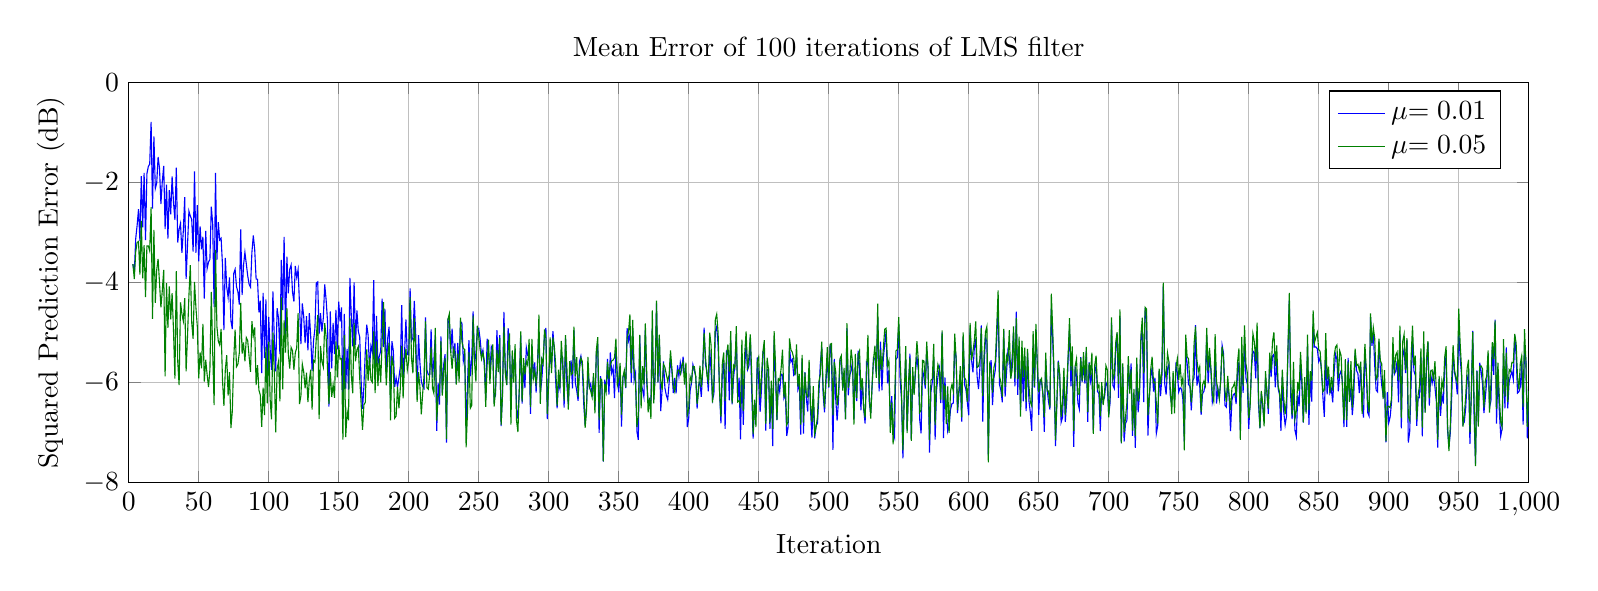
\begin{tikzpicture}

\begin{axis}[%
width=7in,
height=2in,
unbounded coords=jump,
scale only axis,
xmin=0,
xmax=1000,
xlabel={Iteration},
xmajorgrids,
ymin=-8,
ymax=0,
ylabel={Squared Prediction Error (dB)},
ymajorgrids,
title={Mean Error of 100 iterations of LMS filter},
legend style={draw=black,fill=white,legend cell align=left}
]
\addplot [color=blue,solid]
  table[row sep=crcr]{1	-inf\\
2	-inf\\
3	-3.63247548635504\\
4	-3.81027336542774\\
5	-3.12397691635872\\
6	-2.86119902064024\\
7	-2.53539684624931\\
8	-3.16676112268411\\
9	-1.87287963215152\\
10	-2.89688874222132\\
11	-1.80683447738346\\
12	-3.15464147007006\\
13	-1.82458327166948\\
14	-1.68218341073531\\
15	-1.63219789029952\\
16	-0.789873205247798\\
17	-2.52106072520631\\
18	-1.07635051731517\\
19	-2.12206374118726\\
20	-2.01047389834986\\
21	-1.49122357115496\\
22	-1.71447323590754\\
23	-2.42978853845123\\
24	-1.97543467466643\\
25	-1.67025813003234\\
26	-2.93089159099133\\
27	-2.04522139840017\\
28	-3.12381120028265\\
29	-2.15094901863687\\
30	-2.63505146356142\\
31	-1.87654503355272\\
32	-2.40262454377799\\
33	-2.7453475377885\\
34	-1.70088815294819\\
35	-3.19969168180634\\
36	-2.93538290069497\\
37	-2.81850679309292\\
38	-3.40593451015415\\
39	-2.97247798300073\\
40	-2.29111148470788\\
41	-3.92961782112619\\
42	-3.2598771586991\\
43	-2.57312199597864\\
44	-2.6698027618443\\
45	-2.73772306419399\\
46	-3.38216149089385\\
47	-1.7790567708878\\
48	-3.40601930425312\\
49	-2.45302270596887\\
50	-3.57691924870831\\
51	-2.87609797021169\\
52	-3.33570399128563\\
53	-3.08634697136012\\
54	-4.32247938157095\\
55	-2.96737516540653\\
56	-3.72326186941555\\
57	-3.59225336331484\\
58	-3.53905369715812\\
59	-2.48300424488342\\
60	-2.83484090695784\\
61	-4.49323109552297\\
62	-1.80790535669003\\
63	-3.54664196586379\\
64	-2.79275260967805\\
65	-3.15011448081517\\
66	-3.11598806703742\\
67	-3.6573829516309\\
68	-4.95268126957554\\
69	-3.50699770282685\\
70	-4.08799294216062\\
71	-4.29688941353878\\
72	-3.89856645447646\\
73	-4.76802800766952\\
74	-4.93285534162118\\
75	-3.81858257054167\\
76	-3.73662037444284\\
77	-4.08548666300303\\
78	-4.18449976039462\\
79	-4.44116335745449\\
80	-2.93965241749831\\
81	-4.24994426140523\\
82	-3.65904327453896\\
83	-3.39631035497168\\
84	-3.63029550539749\\
85	-3.86495830784621\\
86	-4.03579420976777\\
87	-4.09389458851054\\
88	-3.39546083627826\\
89	-3.06073325420393\\
90	-3.34518353549231\\
91	-3.9297234247452\\
92	-3.93591588076783\\
93	-4.59797380803468\\
94	-4.36193585400703\\
95	-5.81414545625924\\
96	-4.21003660536929\\
97	-5.51335235439191\\
98	-4.33995258796265\\
99	-5.94677100557913\\
100	-4.68788203220713\\
101	-5.32755486052862\\
102	-5.74994291163314\\
103	-4.17794058791482\\
104	-5.12754921609625\\
105	-5.77603347215157\\
106	-4.51314193359643\\
107	-4.71655557395317\\
108	-5.43301507578552\\
109	-3.54677166767047\\
110	-4.55415045099688\\
111	-3.08959662509114\\
112	-5.09745107089481\\
113	-3.4845546165726\\
114	-4.21639451783591\\
115	-3.73867758308483\\
116	-3.64946577428094\\
117	-4.19197457190497\\
118	-4.38341255737077\\
119	-3.66817467723873\\
120	-3.89816782030446\\
121	-3.7417274362719\\
122	-4.44215084486499\\
123	-5.23098015147528\\
124	-4.42082029417066\\
125	-4.67937965833079\\
126	-5.21045434660141\\
127	-4.672824558333\\
128	-5.3564470644181\\
129	-4.61557273509152\\
130	-5.07976867749425\\
131	-5.76993096063825\\
132	-5.17129559850032\\
133	-4.92355279811779\\
134	-4.01040597920574\\
135	-3.98708215533431\\
136	-5.03004173386208\\
137	-4.61598643906784\\
138	-4.98079675101542\\
139	-4.71236782097727\\
140	-4.04017591230564\\
141	-4.34323928682154\\
142	-4.77373668241086\\
143	-6.48527852730298\\
144	-4.57930871699374\\
145	-5.72007127207096\\
146	-4.81021375980704\\
147	-5.43180297652769\\
148	-4.54783620541458\\
149	-5.33590421980377\\
150	-4.38346842225619\\
151	-4.7798576259146\\
152	-4.49998366094842\\
153	-6.46597255074128\\
154	-4.62758413996881\\
155	-6.12279068351948\\
156	-5.32666086682675\\
157	-6.14326176489467\\
158	-3.90973747569214\\
159	-4.67608219325834\\
160	-5.27596721048848\\
161	-4.00001672868574\\
162	-5.24870722474813\\
163	-4.56010480853413\\
164	-4.97811546379956\\
165	-5.09200892830708\\
166	-5.95600299227652\\
167	-6.52910797356779\\
168	-6.07995648845875\\
169	-5.37865937100885\\
170	-4.84382308987329\\
171	-5.05247089781075\\
172	-5.74358097304372\\
173	-5.26927475423464\\
174	-5.38802607933097\\
175	-3.95085122606293\\
176	-5.92068981391143\\
177	-4.66673401104104\\
178	-5.64147466632448\\
179	-5.47439295810131\\
180	-5.36999949027796\\
181	-4.32344343362547\\
182	-5.29240310919425\\
183	-4.52825290402933\\
184	-5.83082814679367\\
185	-5.11532641306827\\
186	-4.88409276221222\\
187	-6.3077138762551\\
188	-5.17298461247613\\
189	-5.3640911771052\\
190	-6.08540688982492\\
191	-5.90709021487432\\
192	-6.08695057359163\\
193	-5.90276893050681\\
194	-5.68604302300088\\
195	-4.45463296698746\\
196	-5.93974876678861\\
197	-5.43835894566294\\
198	-4.73764074401358\\
199	-5.4402079607979\\
200	-5.44841981372918\\
201	-4.11656485851507\\
202	-5.1662958562123\\
203	-5.10160227378243\\
204	-4.36999677860943\\
205	-5.04048563983235\\
206	-6.25381252875435\\
207	-5.0525225863884\\
208	-5.60385206514297\\
209	-5.97558367999788\\
210	-6.07651272884729\\
211	-6.11757840630343\\
212	-4.70002008212081\\
213	-5.74929133900607\\
214	-5.84656722152092\\
215	-5.83647150154821\\
216	-4.93929297915624\\
217	-5.90126838173844\\
218	-5.5365048619832\\
219	-5.05437309425047\\
220	-6.96626179152201\\
221	-6.01192046341486\\
222	-6.44441141523838\\
223	-5.07908243300136\\
224	-6.2087930351626\\
225	-5.63483911726284\\
226	-5.43516055309898\\
227	-7.20392787829955\\
228	-4.7574906325865\\
229	-4.8091200696672\\
230	-5.40909432443294\\
231	-4.92424679703573\\
232	-5.5080526093555\\
233	-5.20897262479894\\
234	-6.02468654341483\\
235	-5.20617086110806\\
236	-5.65351642229129\\
237	-4.78684841727268\\
238	-4.81326665599696\\
239	-5.5743460697973\\
240	-5.41691249503153\\
241	-6.91370538446049\\
242	-6.061875839186\\
243	-5.1511316638344\\
244	-5.87464942024374\\
245	-5.53889277050666\\
246	-4.5763690643972\\
247	-5.64215698958383\\
248	-5.41075580221806\\
249	-4.9320763881816\\
250	-4.91606843154565\\
251	-5.13095840079967\\
252	-5.45146130304025\\
253	-5.35207893107668\\
254	-5.65180518705798\\
255	-6.30751990415229\\
256	-5.12596046613973\\
257	-5.37884763207993\\
258	-5.81388945073949\\
259	-5.28135623498713\\
260	-5.34922279060619\\
261	-6.33842907869098\\
262	-6.25235907711969\\
263	-4.95443440648462\\
264	-5.68182029936979\\
265	-5.05464073852348\\
266	-6.87084192509041\\
267	-6.18937261920408\\
268	-4.58688547993622\\
269	-5.71807902980792\\
270	-6.05382869171971\\
271	-4.91140917252148\\
272	-5.26549357281651\\
273	-6.46972242455554\\
274	-5.45705209273763\\
275	-5.79666221459682\\
276	-5.34593275536626\\
277	-6.51740719741179\\
278	-6.72466069670623\\
279	-6.13932469343251\\
280	-5.05736854302407\\
281	-6.42240688102698\\
282	-5.7034599544405\\
283	-6.11027609753542\\
284	-5.30015699496514\\
285	-5.45773976323318\\
286	-5.45951753936954\\
287	-6.62597504586006\\
288	-5.26611071094292\\
289	-5.93123064611013\\
290	-5.59673152155914\\
291	-6.20230995348154\\
292	-5.57926599795846\\
293	-4.97240123393268\\
294	-6.21535873184612\\
295	-5.96283713031937\\
296	-5.56194678124242\\
297	-5.06001676896531\\
298	-4.90789199114062\\
299	-6.73116244747968\\
300	-5.81765830569449\\
301	-5.45844721337095\\
302	-5.65755340892651\\
303	-4.97270753649066\\
304	-5.36137363291966\\
305	-5.98692057199177\\
306	-6.51646163144427\\
307	-5.99741160866835\\
308	-6.13053539214444\\
309	-5.44155725405102\\
310	-5.50452308514683\\
311	-6.50085636863276\\
312	-5.12032983757972\\
313	-6.06311931000256\\
314	-6.43278488252198\\
315	-5.79098173834879\\
316	-5.55919966611432\\
317	-6.11996122766985\\
318	-4.95132395774014\\
319	-6.00313422171055\\
320	-6.1602220348549\\
321	-6.36601816220336\\
322	-5.58457874882414\\
323	-5.47092689532269\\
324	-5.68519582545539\\
325	-6.4255179425403\\
326	-6.84869447531696\\
327	-6.46223434443977\\
328	-5.78387785337101\\
329	-6.09748999548839\\
330	-6.02537951398322\\
331	-6.28649029402066\\
332	-5.8893232604956\\
333	-6.49376301322322\\
334	-5.43193568637677\\
335	-5.2302407295576\\
336	-7.00570557536363\\
337	-5.87536850393572\\
338	-6.0921226487413\\
339	-7.58109655238898\\
340	-5.94432538638147\\
341	-6.18749105140354\\
342	-5.53029766925825\\
343	-6.24240935721256\\
344	-5.40091479696601\\
345	-5.81441215853284\\
346	-5.70699074077467\\
347	-6.31059951744851\\
348	-5.27973220765534\\
349	-5.825402471236\\
350	-6.19794906569978\\
351	-5.68930141253321\\
352	-6.88477706480699\\
353	-5.89966485442528\\
354	-5.80134058389781\\
355	-6.11231652828571\\
356	-4.91172358269061\\
357	-5.16701065451307\\
358	-5.03808445509694\\
359	-6.00178866570196\\
360	-4.97053891744597\\
361	-5.95606090873082\\
362	-5.8111968640196\\
363	-6.97962646432131\\
364	-7.14880859239347\\
365	-5.06203052550191\\
366	-6.03979792951178\\
367	-6.13740076009599\\
368	-6.28895286423998\\
369	-4.94711603784657\\
370	-6.00153211093415\\
371	-6.37783709932104\\
372	-6.35911309946962\\
373	-6.39520909302748\\
374	-4.91136267659422\\
375	-6.34196789836228\\
376	-5.78340049334494\\
377	-4.41686840319429\\
378	-6.00127234156922\\
379	-5.1141031730738\\
380	-6.57100194299706\\
381	-6.13634796443801\\
382	-5.58046130600922\\
383	-6.11080605597553\\
384	-6.25608900106351\\
385	-6.34280374332207\\
386	-6.01174976299095\\
387	-5.5059226256015\\
388	-5.77302797820211\\
389	-6.21174951131468\\
390	-5.91036142811176\\
391	-6.21643923907596\\
392	-5.65643602660234\\
393	-5.87625378558044\\
394	-5.60041980525291\\
395	-5.76400979970937\\
396	-5.48623029879221\\
397	-5.86728676096359\\
398	-5.81833247417846\\
399	-6.89375728075455\\
400	-6.71498490904695\\
401	-6.16610919326677\\
402	-6.01086063111315\\
403	-5.64430641252916\\
404	-5.7610198928047\\
405	-5.8740071045948\\
406	-6.52151622009926\\
407	-6.06152231702222\\
408	-5.99021615435154\\
409	-6.28909506034876\\
410	-5.75547907067113\\
411	-4.9055496271277\\
412	-5.64270422939714\\
413	-5.77462942933873\\
414	-6.17549397535771\\
415	-5.34637841579887\\
416	-5.77377750347591\\
417	-6.34638851094845\\
418	-6.22412640472565\\
419	-4.98395223421248\\
420	-4.88169346965297\\
421	-5.26053048186927\\
422	-6.13356387099421\\
423	-6.81881436562496\\
424	-5.85263847271346\\
425	-5.60710413751546\\
426	-6.92784871582064\\
427	-5.36885213210432\\
428	-5.35918219159089\\
429	-6.35851630662552\\
430	-5.15577455148012\\
431	-6.43602507341487\\
432	-5.91122540285455\\
433	-5.6364607465899\\
434	-5.07845149596862\\
435	-6.37044113491345\\
436	-5.90144383978427\\
437	-7.13619864648198\\
438	-5.66198560617958\\
439	-6.84829185614004\\
440	-5.69565184712314\\
441	-5.21038905448158\\
442	-5.74602603623736\\
443	-5.67009257552157\\
444	-5.09209003769615\\
445	-6.1675246236771\\
446	-7.12077860768153\\
447	-6.42466819342001\\
448	-6.69990301352987\\
449	-5.49662201089366\\
450	-5.98049972875489\\
451	-6.58643024206819\\
452	-6.12921408571996\\
453	-5.39509395956034\\
454	-5.41544679155032\\
455	-6.96305649540073\\
456	-5.74973808989141\\
457	-5.73245181455563\\
458	-6.92697545622467\\
459	-6.10803632933234\\
460	-7.27309401246576\\
461	-5.15295549463687\\
462	-5.87738095140143\\
463	-6.75307020766797\\
464	-6.02152277365841\\
465	-6.18464520202824\\
466	-5.83297861646135\\
467	-5.84932372358368\\
468	-6.30444044495689\\
469	-6.17590548351343\\
470	-7.06918035909515\\
471	-6.89692485437916\\
472	-5.30846902168894\\
473	-5.58900331463406\\
474	-5.53860472488627\\
475	-5.85581055966173\\
476	-5.824231791114\\
477	-5.42836883273495\\
478	-6.13011220102129\\
479	-6.01115286089343\\
480	-7.04310464274\\
481	-5.52677720408393\\
482	-7.02307572053903\\
483	-5.79245885749532\\
484	-6.31263365704206\\
485	-6.5796362012121\\
486	-5.72249696455865\\
487	-6.54520196499883\\
488	-7.10231720524289\\
489	-6.26403043413884\\
490	-7.1154193511289\\
491	-6.85659174833723\\
492	-6.81917188104063\\
493	-6.21711589062084\\
494	-5.63133979398266\\
495	-5.29742613307383\\
496	-6.22418579399263\\
497	-6.59700335852655\\
498	-6.03653967691978\\
499	-5.43612592270218\\
500	-6.10434269628614\\
501	-5.24781148954053\\
502	-5.44614687612927\\
503	-7.34982020200827\\
504	-5.52933568388819\\
505	-6.326675793077\\
506	-6.76137270260486\\
507	-6.34975967181399\\
508	-5.55628731536933\\
509	-5.55126236278956\\
510	-6.10512453934419\\
511	-5.85153771926865\\
512	-6.73355266489146\\
513	-4.91302522596299\\
514	-6.25872972120715\\
515	-5.85390798029895\\
516	-5.77280809618789\\
517	-5.58290923083379\\
518	-6.73796474761428\\
519	-5.70644620879392\\
520	-6.3736287267538\\
521	-5.36436900559163\\
522	-5.68746755609784\\
523	-6.5550990413794\\
524	-5.93868619227631\\
525	-6.54168525817138\\
526	-6.82207772560409\\
527	-5.58942137023265\\
528	-5.61769496870355\\
529	-6.39878300512966\\
530	-6.61913805174775\\
531	-6.07485612227207\\
532	-5.50421466224335\\
533	-5.53176848967398\\
534	-5.82703195479079\\
535	-4.70456273525146\\
536	-6.1757407373147\\
537	-5.18485455327379\\
538	-6.1577173589539\\
539	-5.51716832955581\\
540	-5.23061435828839\\
541	-4.97753355090464\\
542	-6.01773456763878\\
543	-5.75352745196735\\
544	-6.88782365157213\\
545	-6.27145004543987\\
546	-6.97837394995824\\
547	-7.09370339450926\\
548	-5.5387802014514\\
549	-5.50049085292688\\
550	-4.84650777288288\\
551	-5.95397129058524\\
552	-6.3353180058916\\
553	-7.51547425421538\\
554	-6.13481855566271\\
555	-5.53282017087052\\
556	-6.9648666470509\\
557	-6.13975448565191\\
558	-5.4256612607448\\
559	-7.14048150888861\\
560	-5.85376275210596\\
561	-6.21724854060614\\
562	-5.77983125934311\\
563	-5.48119846056152\\
564	-5.74963925638512\\
565	-6.74526801597326\\
566	-7.01956432446889\\
567	-5.73933004051956\\
568	-5.89546858283383\\
569	-6.1207004319744\\
570	-5.33657457805159\\
571	-5.72334895352998\\
572	-7.40248423469528\\
573	-6.18917061312388\\
574	-5.98896734506629\\
575	-5.53690506445108\\
576	-7.1423448284013\\
577	-6.16866788620437\\
578	-5.88939190353533\\
579	-5.72222344929627\\
580	-6.41439114053625\\
581	-5.00049349640505\\
582	-7.11397947690353\\
583	-5.90050928566835\\
584	-6.54157057669713\\
585	-6.97705568310344\\
586	-6.86589234475585\\
587	-6.54187499628816\\
588	-6.42457053504033\\
589	-6.4114230361077\\
590	-5.2962836083116\\
591	-5.48256717999719\\
592	-6.61257610730099\\
593	-6.21892756293227\\
594	-5.98489696384457\\
595	-6.78119317053104\\
596	-5.09762347320942\\
597	-6.04194978790732\\
598	-6.14200348359574\\
599	-6.39301384778108\\
600	-6.65464115971776\\
601	-4.92049914334566\\
602	-5.54606165066679\\
603	-5.79922750697102\\
604	-5.3126293645423\\
605	-5.13082944519888\\
606	-5.87982429928959\\
607	-6.12964211588444\\
608	-5.69893304294935\\
609	-4.86012151403314\\
610	-6.78352045181901\\
611	-5.65052200586308\\
612	-5.11120443841917\\
613	-5.18010399577664\\
614	-7.46115513923341\\
615	-5.77076495427348\\
616	-5.55195962584483\\
617	-6.4536510859213\\
618	-5.9094107059921\\
619	-5.74697458070801\\
620	-5.16448896436661\\
621	-4.42115670520035\\
622	-6.04444100975874\\
623	-6.16063773703088\\
624	-6.3971760546261\\
625	-4.96485998476704\\
626	-6.2818008267169\\
627	-5.80346282410655\\
628	-5.36852186001716\\
629	-5.48557382766632\\
630	-5.90725767955326\\
631	-5.50524692888851\\
632	-4.98825223627823\\
633	-6.07821252790799\\
634	-4.58292692799977\\
635	-6.24743901506482\\
636	-5.28734080682964\\
637	-6.54648862576565\\
638	-5.43079225105295\\
639	-6.37854840432809\\
640	-5.47255702376065\\
641	-6.57485270398749\\
642	-5.38154177452882\\
643	-6.36320790433887\\
644	-6.60145995975047\\
645	-6.9676278197242\\
646	-5.2671242270831\\
647	-6.10413190239755\\
648	-4.94343725239886\\
649	-5.63403617124845\\
650	-6.64741388989744\\
651	-5.9600876877849\\
652	-5.99428868444953\\
653	-6.215204867263\\
654	-6.98711499445259\\
655	-5.57496302756643\\
656	-6.12104217292177\\
657	-6.3885358935344\\
658	-6.54209218532554\\
659	-4.50656874627387\\
660	-5.16271177653041\\
661	-5.95144163777092\\
662	-7.27294818648587\\
663	-6.37520729304633\\
664	-5.56587182242826\\
665	-5.89742821364398\\
666	-6.79680628637358\\
667	-6.70075633402208\\
668	-5.91244030494851\\
669	-6.7898571057335\\
670	-6.36078535645132\\
671	-5.52681861022358\\
672	-4.92718885508284\\
673	-6.07813866828076\\
674	-5.50686174348645\\
675	-7.28600010188957\\
676	-5.68106953260364\\
677	-5.86564988205689\\
678	-6.41008778449587\\
679	-6.53007236475366\\
680	-5.49528827577776\\
681	-5.98898810332086\\
682	-5.65207691584034\\
683	-6.02222680964367\\
684	-5.36980001223721\\
685	-6.78814687966414\\
686	-5.59532519676297\\
687	-5.97896220781552\\
688	-5.82892077436857\\
689	-6.96104780539057\\
690	-5.78842561585208\\
691	-5.66406112254214\\
692	-6.18198332340876\\
693	-6.2212699513876\\
694	-6.97222331279329\\
695	-6.07312649574098\\
696	-6.35935335644909\\
697	-6.29811818483387\\
698	-5.99994111690564\\
699	-6.07349494340153\\
700	-6.65108013193634\\
701	-6.39605215951207\\
702	-4.8020983371306\\
703	-6.05896338436931\\
704	-6.12076358618913\\
705	-5.35084821349026\\
706	-5.01641896307579\\
707	-6.30641673241048\\
708	-4.66926820253325\\
709	-7.21702516194913\\
710	-5.69070486469849\\
711	-7.18083500878083\\
712	-6.81910823660167\\
713	-6.75864778401108\\
714	-5.63082222496552\\
715	-6.13650941143135\\
716	-5.61759027876267\\
717	-7.06606306822145\\
718	-6.22883022787847\\
719	-7.3094317332409\\
720	-5.6229116524459\\
721	-6.59544360424135\\
722	-6.23947722331583\\
723	-5.15606740095747\\
724	-4.91368054476909\\
725	-6.39370679885537\\
726	-4.5773779775305\\
727	-4.6704222889557\\
728	-7.06391356781721\\
729	-6.28407641013521\\
730	-5.89874137640082\\
731	-5.70102609961662\\
732	-6.18008516871105\\
733	-5.90595869962509\\
734	-7.02119115397125\\
735	-6.8657560728293\\
736	-5.76533304319806\\
737	-6.27281532018184\\
738	-5.88985225249343\\
739	-4.06180927276411\\
740	-6.02317773143197\\
741	-6.24353560941194\\
742	-5.72504418116686\\
743	-5.63703705932339\\
744	-6.27423759318624\\
745	-6.43993755837229\\
746	-5.92440212243077\\
747	-6.37262669720427\\
748	-5.67022599117987\\
749	-5.8031299207327\\
750	-6.19103204367608\\
751	-6.10373231711261\\
752	-6.13381674287752\\
753	-6.3440716500952\\
754	-7.18736487206945\\
755	-5.42165977900779\\
756	-5.60620274994066\\
757	-6.04298129383705\\
758	-6.0755807971432\\
759	-6.55775602332194\\
760	-5.96793230350398\\
761	-5.90488973840674\\
762	-4.85546147654366\\
763	-6.06306449112622\\
764	-5.88603569654181\\
765	-6.06322995837529\\
766	-6.6471843704442\\
767	-6.22286228496301\\
768	-6.17852469311027\\
769	-6.00195216928563\\
770	-5.08175273864688\\
771	-6.01850542899568\\
772	-5.48956675345489\\
773	-5.75585893040031\\
774	-6.39867781102939\\
775	-6.26901318082382\\
776	-5.39070889976995\\
777	-6.4199359376635\\
778	-6.12783147858921\\
779	-6.30152828440066\\
780	-5.97215155652648\\
781	-5.25719934624094\\
782	-5.41664963352518\\
783	-6.45789215338486\\
784	-6.49320472422084\\
785	-6.0380520200276\\
786	-6.28039142915391\\
787	-6.97252087648506\\
788	-6.35558595528997\\
789	-6.24361585566343\\
790	-6.21908359853896\\
791	-6.43003337941778\\
792	-5.82187673434182\\
793	-5.59603516534544\\
794	-6.96525734775948\\
795	-5.46105585032744\\
796	-6.20968034341986\\
797	-5.13727582302848\\
798	-5.90552528526303\\
799	-6.03527533083276\\
800	-6.92721378265264\\
801	-6.38928446326874\\
802	-5.70275570968429\\
803	-5.37242475341933\\
804	-5.40432598484521\\
805	-5.91520687225059\\
806	-5.04118151918686\\
807	-6.4186047873483\\
808	-6.9151814064783\\
809	-6.21950951453253\\
810	-6.46076483215274\\
811	-6.78620832107112\\
812	-5.90154750548747\\
813	-6.14595702023732\\
814	-6.62861889489512\\
815	-5.4987557472885\\
816	-5.89112451646117\\
817	-5.46974958851425\\
818	-5.4364573559944\\
819	-6.09912652648334\\
820	-5.52995688580734\\
821	-6.12380047237129\\
822	-6.24209330585443\\
823	-6.96688296896183\\
824	-5.87346617068868\\
825	-6.58380273040708\\
826	-6.85087903593208\\
827	-6.67327503388229\\
828	-5.40701945748833\\
829	-4.35529777335928\\
830	-6.2879449279998\\
831	-6.7332851421464\\
832	-6.04648883595409\\
833	-6.95293049780722\\
834	-7.08296821639256\\
835	-6.25895263082019\\
836	-6.47649843701908\\
837	-5.61626204444931\\
838	-6.06812249246004\\
839	-6.80441042314263\\
840	-6.00477608086912\\
841	-6.58643463191813\\
842	-5.27518037613553\\
843	-6.84596303196633\\
844	-5.82767073782714\\
845	-6.38196483328236\\
846	-4.83258739850024\\
847	-5.29055443521375\\
848	-5.28965261428229\\
849	-5.32733508629758\\
850	-5.5837292588711\\
851	-5.50019842414557\\
852	-5.75860672540543\\
853	-6.29663858921381\\
854	-6.68664172664437\\
855	-5.50987739754762\\
856	-6.23781737663835\\
857	-5.82768307134338\\
858	-6.21190294053101\\
859	-6.12792566925683\\
860	-6.39865768591369\\
861	-5.79650265267622\\
862	-5.43617623219487\\
863	-5.5404933675436\\
864	-6.17664360408119\\
865	-5.83914799113733\\
866	-5.76522228457586\\
867	-6.0052739236371\\
868	-6.89348034695299\\
869	-5.8040733108294\\
870	-6.88551982154821\\
871	-5.50750866587225\\
872	-6.37253499176539\\
873	-6.11351391209918\\
874	-6.65347726231413\\
875	-6.30281183111211\\
876	-5.40872722873813\\
877	-5.76057076548415\\
878	-5.82302733359215\\
879	-6.21183759723527\\
880	-5.69583560654253\\
881	-6.46312857378496\\
882	-6.70121447042562\\
883	-5.43626718531002\\
884	-5.79057738955141\\
885	-6.60246190881746\\
886	-6.6728246082295\\
887	-4.69196939523041\\
888	-5.26541710774586\\
889	-4.99060006628795\\
890	-5.66722501905019\\
891	-6.1507746180854\\
892	-6.18704964129023\\
893	-5.18070487409763\\
894	-5.71578347642196\\
895	-6.05751008475486\\
896	-6.25506070392434\\
897	-6.08260734848763\\
898	-7.19989565367109\\
899	-6.19236047420437\\
900	-6.80818100523333\\
901	-6.69337949049787\\
902	-6.39724448307126\\
903	-5.37226328676958\\
904	-5.83616006342821\\
905	-5.77180132265658\\
906	-5.57301173619454\\
907	-6.39534126778984\\
908	-5.03182477584246\\
909	-6.91790188120196\\
910	-5.47036126034754\\
911	-5.33025071943224\\
912	-5.81192717552259\\
913	-5.15238408612949\\
914	-7.20102593553571\\
915	-6.9778380630075\\
916	-6.00025787430672\\
917	-5.13935188020784\\
918	-5.76847839525113\\
919	-5.85778070825993\\
920	-6.86878302341119\\
921	-6.29979244702841\\
922	-6.30567729476315\\
923	-5.48177632827677\\
924	-7.07615802468135\\
925	-5.28468999021742\\
926	-6.58537790014163\\
927	-5.70220026986629\\
928	-5.19755927122354\\
929	-6.46104853081431\\
930	-5.84350792612125\\
931	-6.01540293733664\\
932	-5.84378455295344\\
933	-6.09386673180217\\
934	-6.37887084266446\\
935	-7.30440397819043\\
936	-5.92751461771309\\
937	-6.66615645427016\\
938	-6.22948009333059\\
939	-6.4214470906651\\
940	-5.69978200012693\\
941	-5.45649318497096\\
942	-6.94124698270518\\
943	-7.28921907678941\\
944	-7.00510346842878\\
945	-6.27243560878351\\
946	-5.41168322939593\\
947	-5.80442989121634\\
948	-5.95033557938057\\
949	-6.23872553607529\\
950	-4.91453347029086\\
951	-5.50315268885539\\
952	-5.84208870649835\\
953	-6.83759865217985\\
954	-6.79018976659876\\
955	-6.50432299641127\\
956	-5.96118683840667\\
957	-5.80793018159071\\
958	-7.2302249522258\\
959	-6.17696998717156\\
960	-4.97058125065142\\
961	-6.72691835097161\\
962	-7.62372507819108\\
963	-5.76007136797031\\
964	-6.80016805567325\\
965	-5.60648036291077\\
966	-5.77733391903957\\
967	-6.02830255308269\\
968	-6.61342201203019\\
969	-6.30124176722654\\
970	-5.97523651681753\\
971	-5.44051353859727\\
972	-6.49894726325563\\
973	-6.37288745284355\\
974	-5.27239879412615\\
975	-5.84727344887736\\
976	-4.7419570416948\\
977	-6.82102824699607\\
978	-5.80316235122179\\
979	-6.56987904385906\\
980	-7.07410782444692\\
981	-6.91770132847532\\
982	-5.42759795989927\\
983	-6.51573027047077\\
984	-5.30051049371916\\
985	-6.51835217068514\\
986	-5.98992697507144\\
987	-5.87158626693601\\
988	-5.77715192271757\\
989	-5.93822176679148\\
990	-5.06279559788093\\
991	-5.45235095708737\\
992	-6.21331208902013\\
993	-6.18582277676573\\
994	-6.08684895406409\\
995	-5.5778689960858\\
996	-6.84472303578738\\
997	-5.25312305571247\\
998	-5.54766143796934\\
999	-7.11900327277395\\
1000	-6.38300967321852\\
};
\addlegendentry{$\mu\text{ = 0.01}$};

\addplot [color=black!50!green,solid]
  table[row sep=crcr]{1	-inf\\
2	-inf\\
3	-3.63247548635504\\
4	-3.93028659363022\\
5	-3.38906828690839\\
6	-3.20096130844574\\
7	-3.1799134360866\\
8	-3.8411935954528\\
9	-2.76639402529972\\
10	-3.91646665987112\\
11	-3.25229787451263\\
12	-4.29230478496534\\
13	-3.2686520718288\\
14	-3.26778335594379\\
15	-3.36998270300881\\
16	-2.49072910880358\\
17	-4.72939513502913\\
18	-2.94863907720311\\
19	-4.4062529593115\\
20	-3.74882851815183\\
21	-3.52677260593842\\
22	-4.00509379579197\\
23	-4.49894850018756\\
24	-4.15786887366633\\
25	-3.74634518348942\\
26	-5.8759912333005\\
27	-4.01485849245513\\
28	-4.90700371212194\\
29	-4.07623403615972\\
30	-4.73756018446936\\
31	-4.21140775503519\\
32	-4.96554007423545\\
33	-5.92272997038101\\
34	-3.7735315490843\\
35	-5.57199863189526\\
36	-6.05353686941499\\
37	-4.39639913545874\\
38	-4.62891382672662\\
39	-4.77278588201405\\
40	-4.31182596731614\\
41	-5.77596260014775\\
42	-5.07738431935242\\
43	-4.26932702816833\\
44	-3.65540031457605\\
45	-4.80023416407126\\
46	-5.12812701148441\\
47	-3.9884074720239\\
48	-4.49906530291408\\
49	-4.87906754423568\\
50	-5.91758741804308\\
51	-5.39850783657477\\
52	-5.71577558205681\\
53	-4.82922907207079\\
54	-5.98059490885657\\
55	-5.54628081588448\\
56	-5.83959493917543\\
57	-6.09250462545014\\
58	-5.74234622327775\\
59	-4.18869478365115\\
60	-5.40484709948711\\
61	-6.45200706741968\\
62	-3.34849288436566\\
63	-4.88068689496432\\
64	-5.17317210728726\\
65	-5.25054554280326\\
66	-4.92877652466621\\
67	-5.95854684438848\\
68	-6.46504676207756\\
69	-5.75016641743878\\
70	-5.45602325071244\\
71	-6.26354896201767\\
72	-5.79379038385281\\
73	-6.9106790294446\\
74	-6.57517905451608\\
75	-5.54644451574626\\
76	-4.94452618807657\\
77	-5.68430160297296\\
78	-5.63348679557136\\
79	-5.40923731381229\\
80	-4.40854877598435\\
81	-5.42416794736867\\
82	-5.20097340024252\\
83	-5.57823942306281\\
84	-5.1026414280806\\
85	-5.16403271983014\\
86	-5.47833428143875\\
87	-5.78693839015873\\
88	-4.77322623076562\\
89	-5.06462916828914\\
90	-4.90087513356805\\
91	-6.0524016895811\\
92	-5.65326835005265\\
93	-6.15264052723612\\
94	-6.25218793883051\\
95	-6.88519384128132\\
96	-6.10514788638992\\
97	-6.65160099589965\\
98	-5.28948513416024\\
99	-6.41562550175724\\
100	-5.1848182567426\\
101	-6.3295611439698\\
102	-6.73711622899615\\
103	-5.00051433896939\\
104	-5.78680779496003\\
105	-6.9953621916114\\
106	-5.7255271373439\\
107	-5.57926128567525\\
108	-6.37610987216946\\
109	-4.29810968247667\\
110	-6.13738807042615\\
111	-4.76056476217393\\
112	-5.40171721836983\\
113	-4.51452854325378\\
114	-5.4241436018158\\
115	-5.7219943534307\\
116	-5.30000992072075\\
117	-5.36552853916528\\
118	-5.74657624021885\\
119	-5.40516414429055\\
120	-5.30847041723988\\
121	-4.61388747282615\\
122	-6.43195788277837\\
123	-6.26589858739295\\
124	-5.63172662664294\\
125	-5.78662445868094\\
126	-6.11817619523031\\
127	-5.8054515638521\\
128	-6.39137999177725\\
129	-5.95541138763851\\
130	-5.74407625116906\\
131	-6.54267326505262\\
132	-5.5570630188789\\
133	-5.59532305323589\\
134	-5.11231891265407\\
135	-4.64779688152717\\
136	-6.73186347472795\\
137	-5.27093215106855\\
138	-5.58083441785007\\
139	-5.68849649272279\\
140	-4.81316052872865\\
141	-5.08443111221023\\
142	-5.7243221558005\\
143	-6.42695107724219\\
144	-5.7881540267467\\
145	-6.28953774750333\\
146	-6.046525837989\\
147	-6.30861723778736\\
148	-5.17671686757354\\
149	-5.89628685985926\\
150	-5.26088164364936\\
151	-5.53182543191309\\
152	-5.52338308995265\\
153	-7.14348322672885\\
154	-5.05514508380267\\
155	-7.09226274918771\\
156	-6.57543110099485\\
157	-6.75542759503891\\
158	-4.70416215750174\\
159	-5.84879518911445\\
160	-6.2149492439014\\
161	-4.80604466627498\\
162	-5.57605043819629\\
163	-5.34814391918209\\
164	-5.28339030848275\\
165	-5.91575130331175\\
166	-6.41885544093523\\
167	-6.9476827793233\\
168	-6.44602955033633\\
169	-6.39756779982259\\
170	-5.33708557151544\\
171	-5.96976968717156\\
172	-5.50077597499423\\
173	-5.94845843315887\\
174	-5.99435711500244\\
175	-4.97981226533619\\
176	-6.21023532888442\\
177	-5.17934320500473\\
178	-6.0739461492384\\
179	-5.51688416548997\\
180	-5.99821203338332\\
181	-5.17287186194709\\
182	-4.39507160475776\\
183	-5.30558636485493\\
184	-6.05721317844931\\
185	-5.48245686317639\\
186	-5.20162545217404\\
187	-6.75769836702351\\
188	-5.46816455948428\\
189	-5.6488512920295\\
190	-6.71263559201828\\
191	-6.67257859895918\\
192	-6.08919768069271\\
193	-6.51532150130253\\
194	-6.11732782327673\\
195	-5.26754959053784\\
196	-6.31763560786637\\
197	-5.62593893981551\\
198	-5.32303318827253\\
199	-5.74824372840492\\
200	-5.57074330041876\\
201	-4.29264954197771\\
202	-5.51976186769202\\
203	-5.81471166165186\\
204	-4.71099451274104\\
205	-5.36479049706896\\
206	-6.38652125338454\\
207	-5.79250764289614\\
208	-6.08056981228341\\
209	-6.63882547588169\\
210	-6.20582820788112\\
211	-5.85495334776362\\
212	-4.77835101822168\\
213	-6.10321765194908\\
214	-6.13461222687554\\
215	-5.84085969094865\\
216	-5.29028521908322\\
217	-6.11651087035858\\
218	-6.21942108563248\\
219	-4.90896219360925\\
220	-6.76301994507341\\
221	-6.28417116999555\\
222	-6.26068756515912\\
223	-5.17062149740987\\
224	-6.26106646131888\\
225	-5.79465756147862\\
226	-5.5103116995975\\
227	-7.13259730357938\\
228	-4.74173784723353\\
229	-4.62815609679215\\
230	-5.38639702868585\\
231	-5.72862369462379\\
232	-5.32342147520553\\
233	-5.40864093527106\\
234	-6.04337500987364\\
235	-5.4234012754691\\
236	-5.99862369880349\\
237	-4.70515998224652\\
238	-5.18271514834428\\
239	-5.31846677137453\\
240	-5.3387819869259\\
241	-7.29830969475388\\
242	-6.59090104968567\\
243	-5.39076769524529\\
244	-6.51355842689069\\
245	-6.45722717174225\\
246	-4.66499732161625\\
247	-5.58631123981486\\
248	-5.98453595373271\\
249	-4.86299526128202\\
250	-5.08839764470929\\
251	-5.34251790991858\\
252	-5.52862045768518\\
253	-5.40358993176455\\
254	-5.56569691970412\\
255	-6.48854911020409\\
256	-5.66102002844479\\
257	-5.14138548467787\\
258	-6.02930782958613\\
259	-5.50243874530256\\
260	-5.23753113213983\\
261	-6.48352342811788\\
262	-6.15729129569109\\
263	-5.34677446317179\\
264	-5.79048249323311\\
265	-5.10605963237236\\
266	-6.85105697208859\\
267	-6.2576213562575\\
268	-4.88460710620218\\
269	-5.82063592648956\\
270	-6.04928940164222\\
271	-5.37281078415232\\
272	-5.01786969325577\\
273	-6.84172961115941\\
274	-5.35800862352387\\
275	-6.00184690037139\\
276	-5.23351015386096\\
277	-6.75887313492874\\
278	-6.98958693902922\\
279	-6.11980835715528\\
280	-4.97946820651366\\
281	-6.38321950162158\\
282	-5.51557356267781\\
283	-5.83999087944659\\
284	-5.57332454305296\\
285	-5.65476008539224\\
286	-5.12861883387384\\
287	-6.49160346936828\\
288	-5.12928183737135\\
289	-5.93119996255456\\
290	-5.77365569509358\\
291	-6.02437001662445\\
292	-5.75492350797365\\
293	-4.64077640357965\\
294	-6.42796251820205\\
295	-5.53193141845575\\
296	-5.62122622995074\\
297	-4.93907024008317\\
298	-5.12131071299591\\
299	-6.63389364097133\\
300	-6.00060051770233\\
301	-5.09855214615357\\
302	-5.81499985522088\\
303	-5.10018400914629\\
304	-5.28014422930329\\
305	-5.65492192317133\\
306	-6.46824427907184\\
307	-5.74173248916851\\
308	-6.11103191726202\\
309	-5.16635551396545\\
310	-5.66109787772452\\
311	-6.36162242986769\\
312	-5.05373715899431\\
313	-5.70669599904397\\
314	-6.54052703964541\\
315	-5.57417513578825\\
316	-5.84775072885496\\
317	-5.81723100183329\\
318	-4.88463505251648\\
319	-5.87759078014643\\
320	-5.49422116047703\\
321	-6.29281502575405\\
322	-5.74146699452987\\
323	-5.50896029857559\\
324	-5.58106254212158\\
325	-6.1276205462382\\
326	-6.90856847097983\\
327	-6.56523367616754\\
328	-5.48962155051877\\
329	-6.08360256456374\\
330	-6.17439747850582\\
331	-6.29342463516783\\
332	-5.81143536248141\\
333	-6.61948803315967\\
334	-5.35907962758249\\
335	-5.0953618233182\\
336	-6.75462552403279\\
337	-5.92637791488926\\
338	-5.95159790571864\\
339	-7.57773157165751\\
340	-6.0284267737595\\
341	-6.1847899087875\\
342	-5.58711341464893\\
343	-5.93721936413093\\
344	-5.63614327588569\\
345	-5.56884377927382\\
346	-5.55168015265179\\
347	-5.50489054740723\\
348	-5.1218441926151\\
349	-6.05985377002998\\
350	-5.94122166395532\\
351	-5.61027271232337\\
352	-6.64224909226435\\
353	-5.89122401384132\\
354	-5.76219789929538\\
355	-6.09645515602992\\
356	-5.10810143102098\\
357	-4.99149166836158\\
358	-4.6369233454911\\
359	-5.810015284363\\
360	-4.75049980588401\\
361	-5.72972793713423\\
362	-6.01342418732489\\
363	-6.89224937588026\\
364	-6.66967412640513\\
365	-5.04992430424433\\
366	-6.51789965930254\\
367	-5.67438226154878\\
368	-6.04320168406527\\
369	-4.82027023287258\\
370	-5.78468733725886\\
371	-6.59652534065219\\
372	-6.3023580827541\\
373	-6.72610679844042\\
374	-4.55763308595753\\
375	-6.41820038746309\\
376	-5.92495652937932\\
377	-4.36501494757262\\
378	-5.9901639028614\\
379	-5.04253347209522\\
380	-5.95411983400138\\
381	-6.14650107397097\\
382	-5.6360811093538\\
383	-5.69787794528265\\
384	-5.8365150626281\\
385	-5.97351180195757\\
386	-5.844710257992\\
387	-5.35625632240741\\
388	-5.73270890653683\\
389	-6.0635835841632\\
390	-6.17781443595822\\
391	-5.93095046078075\\
392	-5.77010472023429\\
393	-5.74740471563124\\
394	-5.83039016081993\\
395	-5.66604323280414\\
396	-5.58908357990671\\
397	-6.04264404133993\\
398	-5.60331445162795\\
399	-6.65648429835236\\
400	-6.53334332208733\\
401	-5.88246242871298\\
402	-5.97262933854433\\
403	-5.67734314061533\\
404	-5.68284999122\\
405	-5.87600037654668\\
406	-6.42859464384797\\
407	-6.18446287225419\\
408	-5.66303025619161\\
409	-6.0925460368697\\
410	-5.74332847191535\\
411	-5.00386003509483\\
412	-5.49200551993999\\
413	-5.85115071007591\\
414	-5.97240045419217\\
415	-5.00171090860704\\
416	-5.2624344806738\\
417	-6.40207495140768\\
418	-5.96927840468635\\
419	-4.74023322400755\\
420	-4.63507387777104\\
421	-5.00381714101035\\
422	-6.17042404335095\\
423	-6.68784663241705\\
424	-5.61935380527209\\
425	-5.40128240165315\\
426	-6.37370032317437\\
427	-5.46114636379135\\
428	-5.24121934257796\\
429	-5.78444786617469\\
430	-4.97209745511821\\
431	-6.41873536783142\\
432	-5.65792812818747\\
433	-5.71456362569001\\
434	-4.87471407187461\\
435	-6.38843528177793\\
436	-6.36587238857671\\
437	-6.46276884178346\\
438	-5.14092128455536\\
439	-6.56769886581439\\
440	-5.42128240503571\\
441	-4.97933241221514\\
442	-5.74804367158861\\
443	-5.48974199682965\\
444	-5.03604147377067\\
445	-5.82402310077988\\
446	-7.0356737752283\\
447	-6.34158631101927\\
448	-6.89028683966744\\
449	-5.57707258554958\\
450	-5.49134462365718\\
451	-6.3084085575177\\
452	-5.86623094542331\\
453	-5.38665300691802\\
454	-5.15357037168962\\
455	-6.82461324453152\\
456	-5.5060007998698\\
457	-5.74458328983247\\
458	-6.80172761320365\\
459	-5.96142320466536\\
460	-6.930615649499\\
461	-4.97319213184024\\
462	-5.6367431618746\\
463	-6.75168562168689\\
464	-5.92552573090754\\
465	-5.95953368366395\\
466	-5.71896009344645\\
467	-5.34455135727099\\
468	-6.30098977253259\\
469	-5.98676010836151\\
470	-6.84469950734206\\
471	-6.7946707622873\\
472	-5.11967930141948\\
473	-5.34411207876749\\
474	-5.39712921940337\\
475	-5.51027449327236\\
476	-5.85795731456803\\
477	-5.24003744795011\\
478	-6.08316928928071\\
479	-5.82691783110199\\
480	-6.8410772181253\\
481	-5.44968652356577\\
482	-6.80027212981801\\
483	-5.80381276021738\\
484	-6.23703839087407\\
485	-6.28609516052754\\
486	-5.55006691516171\\
487	-6.42781321408049\\
488	-6.79649437782634\\
489	-6.07438096419925\\
490	-7.02530497107201\\
491	-6.89765875344098\\
492	-6.67469811812074\\
493	-5.98475244003762\\
494	-5.83413643691855\\
495	-5.1830109254646\\
496	-6.10082585756462\\
497	-6.5043979608508\\
498	-5.88995958227335\\
499	-5.29108293970541\\
500	-6.08847933965578\\
501	-5.23415616504779\\
502	-5.22074998158755\\
503	-6.65725833764168\\
504	-5.59079685624723\\
505	-5.7880021617467\\
506	-6.45972691839284\\
507	-6.23428263914631\\
508	-5.52967694858582\\
509	-5.46294967697815\\
510	-6.16258931522255\\
511	-5.70600377185205\\
512	-6.73558423269785\\
513	-4.81268080182964\\
514	-6.10632323809382\\
515	-5.88278327007862\\
516	-5.33809594338888\\
517	-5.5886992130418\\
518	-6.84256713598646\\
519	-5.42977980207468\\
520	-6.31429875777884\\
521	-5.45779321873851\\
522	-5.36978924489867\\
523	-6.150081698073\\
524	-5.91650181178095\\
525	-6.516595827787\\
526	-6.70397482501084\\
527	-5.82083772302\\
528	-5.04775223885885\\
529	-6.27706355317956\\
530	-6.72035271285915\\
531	-6.02552601975344\\
532	-5.53567913965799\\
533	-5.26525701921673\\
534	-5.90681960454679\\
535	-4.42315804028319\\
536	-6.03121288662977\\
537	-5.35317241974999\\
538	-5.74800650770961\\
539	-5.33011429229877\\
540	-4.93455691398944\\
541	-4.91447228969348\\
542	-5.6615844538492\\
543	-5.56298926154845\\
544	-7.0095474521566\\
545	-6.40335873680481\\
546	-7.23809651474918\\
547	-6.45894626303098\\
548	-5.36872465338449\\
549	-5.34219034834719\\
550	-4.69231621684581\\
551	-5.53282880571985\\
552	-6.20384684943003\\
553	-7.35633883473333\\
554	-6.24369611466348\\
555	-5.27235327548684\\
556	-7.012170434665\\
557	-6.00448347951426\\
558	-5.50587960916488\\
559	-7.16564469461746\\
560	-5.69162548789179\\
561	-6.24659450068298\\
562	-5.69537833835544\\
563	-5.17409567671141\\
564	-5.55613731121989\\
565	-6.60130701102982\\
566	-6.55624457261674\\
567	-5.55636960753658\\
568	-5.56691931168428\\
569	-6.05252769873087\\
570	-5.18310338139509\\
571	-5.75097829187053\\
572	-7.15455098375893\\
573	-5.95436437888354\\
574	-5.93188682184704\\
575	-5.22692470630446\\
576	-6.8507785994459\\
577	-5.92943739681736\\
578	-5.63866590066761\\
579	-5.73944629434624\\
580	-6.34044888907391\\
581	-4.95743211652241\\
582	-6.35466863004721\\
583	-6.05401021176321\\
584	-6.82955403584135\\
585	-6.07711067738446\\
586	-7.00572655566685\\
587	-6.16819344588398\\
588	-6.04361770772923\\
589	-6.1773031530508\\
590	-5.02381811472531\\
591	-5.52937039870785\\
592	-6.54750100601017\\
593	-6.13713310072378\\
594	-5.6745808939588\\
595	-6.69730289142347\\
596	-4.99635697447382\\
597	-5.8983594204968\\
598	-5.95189226489729\\
599	-6.38282598463267\\
600	-5.88733530781338\\
601	-4.80582497528732\\
602	-5.55851285408657\\
603	-5.38515937193273\\
604	-5.16891898656483\\
605	-4.77948825151057\\
606	-5.69746133092272\\
607	-5.67671584552079\\
608	-5.53009621176655\\
609	-4.90929741374868\\
610	-6.27454891900721\\
611	-5.40703904116442\\
612	-4.98375471755275\\
613	-4.87714865343094\\
614	-7.59602982371947\\
615	-5.64473952041322\\
616	-5.740162612411\\
617	-6.20452046174781\\
618	-5.70189861978897\\
619	-5.58007025811907\\
620	-4.90054612750469\\
621	-4.15729869980721\\
622	-5.87662694981446\\
623	-5.99581613329106\\
624	-6.28480547243039\\
625	-4.93064007397269\\
626	-6.0869335455701\\
627	-5.47236107238725\\
628	-5.58000056362545\\
629	-4.95413823556496\\
630	-5.92392707738455\\
631	-5.75696818964248\\
632	-4.88044057231006\\
633	-5.92393329593107\\
634	-4.70873012372333\\
635	-5.93480983743014\\
636	-5.08357942332395\\
637	-6.68154221705505\\
638	-5.16201070163297\\
639	-5.89972002174614\\
640	-5.30196146361057\\
641	-6.39101062048673\\
642	-5.32638372306104\\
643	-6.07205718545351\\
644	-6.3916309037621\\
645	-6.46800869973346\\
646	-4.97133066686741\\
647	-6.07956014586864\\
648	-4.82987233440812\\
649	-5.65364536056483\\
650	-6.19148034553884\\
651	-5.96437726066616\\
652	-5.91838475388117\\
653	-6.26310661250183\\
654	-6.68763419740371\\
655	-5.40534678373126\\
656	-6.17000284187596\\
657	-6.17015299084768\\
658	-6.49815089396344\\
659	-4.22163475543978\\
660	-4.95060255716629\\
661	-5.82354621160925\\
662	-7.1490141647365\\
663	-6.36440591951567\\
664	-5.58934487810438\\
665	-5.82855583879681\\
666	-6.68689225992693\\
667	-6.4105194080316\\
668	-5.709413367781\\
669	-6.65081383023675\\
670	-6.11332887006041\\
671	-5.46495412816876\\
672	-4.71519577288705\\
673	-5.76104263786249\\
674	-5.27792965759137\\
675	-6.96906951709955\\
676	-5.67336118139914\\
677	-5.52548187827282\\
678	-6.23468190699898\\
679	-6.2285265849171\\
680	-5.50837841756515\\
681	-5.97041276025986\\
682	-5.391406529636\\
683	-5.96091622570025\\
684	-5.28731192440322\\
685	-6.59008739566561\\
686	-5.6162075841487\\
687	-5.80772169290789\\
688	-5.40561782865922\\
689	-7.03006329068556\\
690	-5.65110615951542\\
691	-5.46221976389082\\
692	-6.1161706898285\\
693	-6.04381981187845\\
694	-6.67298195479291\\
695	-5.99348574136147\\
696	-6.45111175487409\\
697	-6.23388372591678\\
698	-5.66242584165242\\
699	-5.74690065715783\\
700	-6.69573618077221\\
701	-6.24890201993783\\
702	-4.69785698077559\\
703	-5.94141110432571\\
704	-5.83956016021874\\
705	-5.19943097287898\\
706	-4.99341390038106\\
707	-6.03387920008117\\
708	-4.53883690387239\\
709	-7.21370856068222\\
710	-5.62013668809679\\
711	-6.99879898418084\\
712	-6.6947068497483\\
713	-6.39633195774015\\
714	-5.47295160330164\\
715	-6.22082007239608\\
716	-5.73808706042804\\
717	-6.96160587450194\\
718	-6.13042393165102\\
719	-7.06618712225473\\
720	-5.50403026035324\\
721	-6.37600856905886\\
722	-6.13886558790766\\
723	-5.05856668185674\\
724	-4.70423967475019\\
725	-5.81812300117436\\
726	-4.49628293464721\\
727	-4.53008949738241\\
728	-6.65531114522112\\
729	-6.31361832636617\\
730	-5.73781508259243\\
731	-5.48624662997832\\
732	-6.00491744339459\\
733	-5.99086430496594\\
734	-6.41500606592412\\
735	-6.82015867493568\\
736	-5.72292880811772\\
737	-6.03025861081665\\
738	-5.76522458706118\\
739	-4.00455222433747\\
740	-5.76207207761783\\
741	-5.91719530668553\\
742	-5.41116388887857\\
743	-5.59054537143651\\
744	-6.1390006078111\\
745	-6.6316247690785\\
746	-5.77122596003607\\
747	-6.61614968753283\\
748	-5.70711008479336\\
749	-5.52405202546012\\
750	-5.94694143443767\\
751	-5.63219783571938\\
752	-6.03283513090458\\
753	-5.89955883899268\\
754	-7.3600621011199\\
755	-5.04175188437213\\
756	-5.48580852822626\\
757	-5.52702585011345\\
758	-6.00472658174301\\
759	-6.39942599133785\\
760	-6.06542983050804\\
761	-5.2103598823698\\
762	-4.88509514216085\\
763	-5.54714875447414\\
764	-5.7837995459444\\
765	-5.68450025838079\\
766	-6.5924421815783\\
767	-6.05229321879372\\
768	-5.97195962634801\\
769	-6.06118453251648\\
770	-4.90801495078162\\
771	-5.77790222915293\\
772	-5.30745654533061\\
773	-5.7139192991729\\
774	-6.22446701802018\\
775	-6.36935611869619\\
776	-5.03171533503317\\
777	-5.98415770729337\\
778	-6.13736868983684\\
779	-6.33705408345045\\
780	-5.93377883901677\\
781	-5.28331570084091\\
782	-5.50455429374762\\
783	-6.16096270459305\\
784	-6.38672650056958\\
785	-5.87078025315294\\
786	-6.24951089073152\\
787	-6.55381916072723\\
788	-6.11693990769837\\
789	-6.07679535077539\\
790	-6.00094229723747\\
791	-6.30057344588479\\
792	-5.60159483833861\\
793	-5.31858815902145\\
794	-7.14719164585224\\
795	-5.08942423987352\\
796	-6.07239281515549\\
797	-4.86039983226244\\
798	-5.62629898925025\\
799	-5.80465446162941\\
800	-6.70854608205477\\
801	-6.47743489644375\\
802	-5.67504801137447\\
803	-5.0237183597929\\
804	-5.19118347705379\\
805	-5.57456667588992\\
806	-4.80298686209419\\
807	-6.24869958397606\\
808	-6.91062014956192\\
809	-6.17050664830787\\
810	-6.41832337629369\\
811	-6.87603046369322\\
812	-5.77183335834645\\
813	-6.23325883193248\\
814	-6.52206264997515\\
815	-5.40272169695974\\
816	-5.7571797847221\\
817	-5.18085687176554\\
818	-4.99657398457151\\
819	-5.67802877863164\\
820	-5.25839554655521\\
821	-6.0606105141337\\
822	-6.19566785651049\\
823	-6.60211020285837\\
824	-5.74250765492219\\
825	-6.30450307607547\\
826	-6.63803502547035\\
827	-6.33786122947384\\
828	-5.36520675685763\\
829	-4.2077473051404\\
830	-5.99331577448285\\
831	-6.66237392871289\\
832	-5.58964797065416\\
833	-6.73061096303248\\
834	-6.575138129698\\
835	-5.98973446924564\\
836	-6.17362906272891\\
837	-5.38869214805438\\
838	-5.91020259095259\\
839	-6.7976623021212\\
840	-5.89257149233636\\
841	-6.62037109469007\\
842	-5.04255746507602\\
843	-6.55459992896915\\
844	-5.77515575111877\\
845	-5.96075449471416\\
846	-4.55793171274441\\
847	-5.1996522687669\\
848	-5.0940278966292\\
849	-4.99756131246302\\
850	-5.34306569592927\\
851	-5.37781463003903\\
852	-5.7959503996915\\
853	-6.18462282086781\\
854	-6.14383870462319\\
855	-5.01128146292335\\
856	-5.93542028027266\\
857	-5.68268347697106\\
858	-6.20852366321391\\
859	-5.89143005355032\\
860	-6.16347714497382\\
861	-5.47309767516281\\
862	-5.29049102581269\\
863	-5.24855424584709\\
864	-5.91982381905808\\
865	-5.36568393153528\\
866	-5.46311784295249\\
867	-6.16636793006016\\
868	-6.75818671845297\\
869	-5.53391347564989\\
870	-6.75285015109044\\
871	-5.58183130765702\\
872	-6.38707519571036\\
873	-5.57094189123107\\
874	-6.50440194579031\\
875	-5.9736578231201\\
876	-5.32440172225187\\
877	-5.65962409937391\\
878	-5.63543698761517\\
879	-5.76014054996418\\
880	-5.58465016125692\\
881	-6.62666792575261\\
882	-5.9670844494285\\
883	-5.22775199534656\\
884	-5.76261497034633\\
885	-6.40744931298454\\
886	-6.59779650684784\\
887	-4.62012676666544\\
888	-5.21126550748183\\
889	-4.90253761056738\\
890	-5.11594309841888\\
891	-5.94550618478716\\
892	-5.8775052615175\\
893	-5.1213186798841\\
894	-5.56166279039743\\
895	-5.62809155645284\\
896	-6.33153192152873\\
897	-5.75220427466908\\
898	-7.17778718599759\\
899	-6.47498516476959\\
900	-6.47898357337839\\
901	-6.50216944612636\\
902	-6.31810402621487\\
903	-5.09384371142588\\
904	-5.81990983141076\\
905	-5.45169929332449\\
906	-5.39179793262328\\
907	-5.95924299881413\\
908	-4.86417368016471\\
909	-6.71219587731814\\
910	-5.17847550378635\\
911	-5.03668213645224\\
912	-5.74657112206068\\
913	-5.11513190554455\\
914	-6.67849603376611\\
915	-6.76203660613203\\
916	-5.48304313670217\\
917	-4.86153897798083\\
918	-5.65520395085313\\
919	-5.46233598059453\\
920	-6.73527691645987\\
921	-6.24976316712089\\
922	-6.06624420230873\\
923	-5.31876316538438\\
924	-6.90339651306718\\
925	-4.97758501399815\\
926	-6.6066082540127\\
927	-5.53006492601161\\
928	-5.17427187310979\\
929	-6.31972054776047\\
930	-5.77148820583899\\
931	-5.75089013813251\\
932	-5.96872922839419\\
933	-5.57533220441805\\
934	-6.14864686581875\\
935	-7.14157817348208\\
936	-5.86843974824657\\
937	-6.47216903350106\\
938	-5.96260689774716\\
939	-6.11890295781318\\
940	-5.48791401487863\\
941	-5.27530085158415\\
942	-6.82529972288808\\
943	-7.3717960908712\\
944	-6.84919987927695\\
945	-5.92736796333695\\
946	-5.25215403795965\\
947	-5.75376850769133\\
948	-5.89975785727876\\
949	-5.99162820061981\\
950	-4.52167036385749\\
951	-5.20733233572743\\
952	-5.71211576365983\\
953	-6.88315270261402\\
954	-6.65671258736002\\
955	-6.26729837303491\\
956	-5.7203713546614\\
957	-5.54644822923989\\
958	-6.99583256198536\\
959	-6.27571603852632\\
960	-4.99283623827519\\
961	-6.37711828686763\\
962	-7.67283906689512\\
963	-5.77300928118847\\
964	-6.88269950109849\\
965	-5.67856801135173\\
966	-5.66912274262413\\
967	-5.72819917009222\\
968	-6.50021693706518\\
969	-5.96350172067787\\
970	-5.87036495215411\\
971	-5.35901304003534\\
972	-6.60192520270683\\
973	-6.01304940700091\\
974	-5.1913915201153\\
975	-5.52575956342705\\
976	-4.76133335146358\\
977	-6.52622079694873\\
978	-5.6031549476047\\
979	-6.30110277143637\\
980	-6.79005479322692\\
981	-6.89056094771211\\
982	-5.1308496237242\\
983	-6.2756668344064\\
984	-5.40530012304561\\
985	-6.39158908410223\\
986	-5.74107902487566\\
987	-5.77968434290063\\
988	-5.59805489372102\\
989	-5.60548862414435\\
990	-5.02857873989449\\
991	-5.21545043407324\\
992	-5.89250603013219\\
993	-6.14250331028649\\
994	-5.61773796753751\\
995	-5.47010785643005\\
996	-6.48613879569587\\
997	-4.93464712199502\\
998	-5.60336993970241\\
999	-6.88934802581138\\
1000	-6.1694282114741\\
};
\addlegendentry{$\mu\text{ = 0.05}$};

\end{axis}
\end{tikzpicture}%}
   	\caption{\textit{LMS filter error (dB) for the given AR process, averaged over 100 independent trials}}
   	\label{fig:q3_1_b}
\end{figure}


\subsubsection{Misadjustment} \label{sec:3_1_c}

Misadjustment is defined as $ \mathcal{M} = \frac{\mathrm{EMSE}}{\sigma^2_\eta}$, where the total mean squared error $ \mathrm{MSE} = \lim_{n \to \infty} \mathbb{E} \{ e^2 (n) \} = \sigma^2_\eta + \mathrm{EMSE} $. Thus we can compute the measured misadjustment from the known mean squared error, and variance of the White Gaussian Noise. We also know that we can approximate $  \mathcal{M} \approx \frac{\mu}{2} \mathbf{Tr} \{ \mathbf{R} \}$ (for small $\mu$) which allows us to have an idea of its theoretical values.

Based on the data obtained in section \ref{sec:3_1_b}, we have taken the mean error squared of the last two hundred samples (when it is known to be in a steady state) across the 100 iterations of the LMS filter, and computed the misadjustment. Table \ref{tab:3_1_c} shows the theoretical and measured misadjustment values. The results are close to the theoretical values, although running the test multiple times does show that the misadjustment varies between each set of 100 trials.

\begin{table}[h]
\centering
\begin{tabular}{|l|l|l|}
\hline	
$\mu$  & Theoretical $\mathcal{M}$ & Measured $\mathcal{M}$ \\ \hline
0.01 & 0.0093                    & 0.0028                 \\ \hline
0.05 & 0.0463                    & 0.0456                 \\ \hline
\end{tabular}
\caption{\textit{Theoretical and Actual Misadjustment values measured for different step sizes}}
\label{tab:3_1_c}
\end{table}

\subsubsection{Steady State Coefficient Values}
By taking the mean of the two hundred last values (when we know the filter is in steady state), and then taking the mean across 100 iterations, we can get estimations of the coefficients $a_1$ and $a_2$. The results are shown in table \ref{tab:3_1_d}. We can see that the coefficient estimates for $\mu = 0.01$ is nearer to the true values than for $\mu = 0.05$. We know that there will always be some error, due to the power of the WGN signal (the $ \sigma^2$ term in the Mean Squared Error equation). We also know from section \ref{sec:3_1_c} that the misadjustment for  $\mu = 0.05$ is larger than for $\mu = 0.01 $, hence it is not surprising that it also less close to the known values than  $\mu = 0.01$. However, we know that a larger step size results in faster convergence to the correct value, so it is a case of a trade off between a small steady state error, and fast convergence.

\begin{table}[h]
\centering
\begin{tabular}{|l|l|l|l|}
\hline
$\mu$ & True Values & 0.05   & 0.01   \\ \hline
$a_1$ & 0.1               & 0.0689 & 0.0943 \\ \hline
$a_2$ & 0.8               & 0.7176 & 0.7691 \\ \hline
\end{tabular}
\caption{\textit{Theoretical and Actual Coefficient values measured for different step sizes}}
\label{tab:3_1_d}
\end{table}

\subsubsection{Leaky LMS Derivation}
In order to derive the leaky LMS equation, we differentiate the given cost function, using the known result of $ \nabla ( e^2(n) ) |_{w_n}$, and that $ \nabla (\lVert \mathbf{x}(n)\rVert_2^2 )|_{x_n} = 2\mathbf{x} $ \cite{Berger2007}  :

\begin{subequations}
\begin{align}
J(n) &= \frac{1}{2} ( e^2(n) + \gamma \lVert \mathbf{w}(n) \rVert_2^2 ) \\
\nabla J(n)|_{w_n} &= \frac{1}{2}  ( \nabla ( e^2(n) ) |_{w_n} + \gamma \nabla (\lVert \mathbf{w}(n)\rVert_2^2 )|_{w_n} ) \\
\nabla J(n)|_{w_n} &= -e(n) \mathbf{x}(n) + \gamma w(n)
\end{align}
\end{subequations}

We then substitute this in to the update function:

\begin{subequations}
\begin{align}
\mathbf{w}(n+1) &= \mathbf{w}[n] + \mu (- \nabla J(n)|_{w_n}) \\
\mathbf{w}(n+1) &= \mathbf{w}[n] + \mu e(n) \mathbf{x}(n) - \mu \gamma \mathbf{w}(n) \\
\mathbf{w}(n+1) &= (1 - \mu \gamma ) \mathbf{w}[n] + \mu e(n) \mathbf{x}(n)
\end{align}
\end{subequations}



\subsubsection{Leaky LMS Results}

Table \ref{tab:3_1_f} shows estimated parameters for $a_1$ and $a_2$ with varying $\mu$ (the same values used in section \ref{sec:3_1_b}) and $\gamma$ values. We can see that as the leakage parameter $\gamma$ increases, the coefficient estimates get progressively less accurate. \cite{Kamenetsky2004} defines $ \lim_{n \to \infty } \mathbb{E}[\mathbf{w}_n] = (\mathbf{R} + \gamma \mathbf{I})^{-1} \mathbf{p} $. The new term added is the $\gamma \mathbf{I} $ term, which effectively introduces noise in to the input matrix $ \mathbf{x} $. Its purpose is to allow the input matrix to have non-zero eigenvalues, as in some cases this can happen, meaning coefficients do not converge. Since the extra term is effectively adding white noise, this explains why the coefficient estimates get progressively worse as $ \gamma $ increases. Since the purpose of Leaky LMS is to help coefficients converge if they otherwise cannot, care should be taken when to add the $ \gamma $ term in, and when it is used to keep it as small as possible, so as to ensure the most accurate results are obtained.

\begin{table}[h]
\centering
\begin{tabular}{|l|l|l|}
\hline
               & $\mu = 0.01 $                  & $\mu = 0.05 $                  \\ \hline
$\gamma = 0$   & $a_1 = 0.0939$, $a_2 = 0.7694$ & $a_1 = 0.0695$, $a_2 = 0.7162$ \\ \hline
$\gamma = 0.2$ & $a_1 = 0.1320$, $a_2 = 0.6078$ & $a_1 = 0.1043$, $a_2 = 0.5463$ \\ \hline
$\gamma = 0.5$ & $a_1 = 0.1412$, $a_2 = 0.4682$ & $a_1 = 0.1105$, $a_2 = 0.4110$ \\ \hline
$\gamma = 0.8$ & $a_1 = 0.1349$, $a_2 = 0.3836$ & $a_1 = 0.1050$, $a_2 = 0.3333$ \\ \hline
\end{tabular}
\caption{\textit{Estimated AR Coefficients for different $\mu$ and $\gamma$}}
\label{tab:3_1_f}
\end{table}

\subsection{Adaptive Step Sizes}

\subsubsection{Implemented GASS Algorithms}
Gradient Adapive Step-Size Algorithms are designed to change the step size as the algorithm progresses. At the start, a large step size is needed in order for the algorithm to converge quickly, but during steady state a small step size helps to reduce the steady state error (as we have observed in previous parts of this coursework).

The LMS algorithm remains the same in structure, but $\mu$ now becomes $\mu(n)$, thus becoming $  \mathbf{w}(n+1) = \mathbf{w}(n) + \mu(n) e(n) \mathbf{x}(n) $. The algorithm to update the weight is defined as $ \mu(n+1) = \mu(n) + \rho e(n) \mathbf{x}^T(n) \psi(n)$. $ \psi(n) $ is defined by three different GASS algorithms, listed below:



\subsubsection{NLMS Algorithm}

The NLMS algorithm is a modification to the LMS algorithm which normalises the power of the input, which for a particularly noisy (in the power spectrum) input signal means the filter can still get to a stable output, which may not happen with a normal LMS filter, or at least not without manually adjusting the step size.

Given the update equation $ \mathbf{w}(n+1) = \mathbf{w}(n) + \mu e_p(n) \mathbf{x}(n) $ and the \textit{a posteriori} relationship given: $  e_p(n) = d(n) - \mathbf{x}^T(n) \mathbf{w}(n+1) $, we can express $ \bigtriangleup \mathbf{w}(n) = \mathbf{w}(n+1) - \mathbf{w}(n) $ to allow us to equate the update equation to the standard NLMS form:

\begin{subequations}
	\begin{align}
	\bigtriangleup \mathbf{w}(n) &= \mathbf{w}(n+1) - \mathbf{w}(n) \\
	\bigtriangleup \mathbf{w}(n) &= \mu e(n) \left[  1 - \mu \frac{\lVert \mathbf{x}(n)\rVert^2}{1 + \mu \lVert \mathbf{x}(n)\rVert^2} \right] \mathbf{x}(n) = \mathbf{w}(n+1) - \mathbf{w}(n) \\
	\bigtriangleup \mathbf{w}(n) &= e(n) \left[ \frac{\mu + \mu^2  \lVert \mathbf{x}(n)\rVert^2 - \mu^2 \lVert \mathbf{x}(n)\rVert^2}{1 + \mu \lVert \mathbf{x}(n)\rVert^2} \right] \mathbf{x}(n) = \mathbf{w}(n+1) - \mathbf{w}(n) \\
	\mathbf{w}(n+1) &= \mathbf{w}(n) + \left[ \frac{1}{\frac{1}{\mu} + \mathbf{x}^T(n)\mathbf{x}(n) } \right] e(n) \mathbf{x}(n)  \label{subeq:3_2_b}
	\end{align}
\end{subequations}

We can see that the last line, equation \ref{subeq:3_2_b} now has the same form (and thus is equivalent to, other than the factors which are discussed below) as the NLMS update equation:
$$ \mathbf{w}(n+1) = \mathbf{w}(n) + \frac{\beta}{\epsilon + \mathbf{x}^T(n)\mathbf{x}(n)} e(n) \mathbf{x}(n) $$

Thus from the comparison of forms, we can equate $ \beta = 1 $ and $ \epsilon = \frac{1}{\mu} $.

\subsubsection{GNGD Algorithm}



%  \begin{figure}[h]
%  	\centering 
% 	\resizebox{0.6\textwidth}{!}{\input{q5/q5_cum.tikz}}
%   	\caption{\textit{Cumulative representation of the variance of each eigenvector}}
%   	\label{fig:q5_4}
%  \end{figure}

% \begin{figure}[h]
% 	\centering 
%  	\setlength\figureheight{0.4\textwidth}
% 	\setlength\figurewidth{0.7\textwidth} 
%  	\input{p_1/1.tikz}
%  	\caption{\textit{The four randomly generated subsets}}
%  	\label{fig:q1}
% \end{figure}


%  \begin{figure}[h]
%          \centering
%          \begin{subfigure}[b]{0.45\textwidth}
%             \resizebox{\textwidth}{!}{\input{part_4/q8_num_1.tikz}}
%   			\caption{\textit{1 Tree}}
%          \end{subfigure}
%          ~ %add desired spacing between images, e. g. ~, \quad, \qquad, \hfill etc.
%           %(or a blank line to force the subfigure onto a new line)
%          \begin{subfigure}[b]{0.45\textwidth}
%             \resizebox{\textwidth}{!}{\input{part_4/q8_num_3.tikz}}
%   			\caption{\textit{2 Trees}}
%          \end{subfigure}
 		
%          \begin{subfigure}[b]{0.45\textwidth}
%             \resizebox{\textwidth}{!}{\input{part_4/q8_num_5.tikz}}
%   			\caption{\textit{5 Trees}}
%          \end{subfigure}
%          ~ %add desired spacing between images, e. g. ~, \quad, \qquad, \hfill etc.
%           %(or a blank line to force the subfigure onto a new line)
%          \begin{subfigure}[b]{0.45\textwidth}
%             \resizebox{\textwidth}{!}{\input{part_4/q8_num_10.tikz}}
%   			\caption{\textit{10 Trees}}
%          \end{subfigure}
         
%          \begin{subfigure}[b]{0.45\textwidth}
%             \resizebox{\textwidth}{!}{\input{part_4/q8_num_20.tikz}}
%   			\caption{\textit{20 Trees}}
%          \end{subfigure}
 		
%  		\label{q9i}
% 		\caption{\textit{Varying the Number of Trees in the Forest}}
%  \end{figure}

\end{document}

